%!TEX root = ../thesis.tex

\chapter{Eigener Ansatz: Social Online Community Connectors (SOCC)} % (fold)
\label{cha:eigener_ansatz_social_online_community_connectors_socc_}

Aufbauend auf den in Kapitel \ref{cha:analyse} identifizierten Komponenten und Wahl der für ein System zur Synchronisation von Beiträgen passenden Techniken, soll nun der als \emph{Social Online Community Connectors} (SOCC) benannter Ansatz vorgestellt werden. Den Aufbau von SOCC ist in Abbildung \ref{fig:uebersicht_socc} zu sehen. Ein \emph{Connector} von SOCC dient dabei als Schnittstelle zwischen den Datenformat der Plattform für die er implementiert wurde und dem SIOC-Format. SOCC stützt sich dabei auf die Prinzipien für die Verbindung von Daten im Web von Tim Berners-Lee (siehe \cite{Berners-Lee2009}):

\begin{description}
    \item[\enquote{Use URIs as names for things}:] Ressourcen wie Seiten, Foren, Threads und Beiträge sollten immer durch eine URI benannt werden.

    \item[\enquote{Use HTTP URIs so that people can look up those names}:] Die verwendeten URIs sollten einer Adresse im Web entsprechen, um auf die dahinter liegenden Daten zugreifen zu können.

    \item[\enquote{When someone looks up a URI, provide useful information, using the standards (RDF*, SPARQL)}:] Die Daten sollten in einen Standard für das Semantic Web formatiert werden. Wie schon erwähnt setzt SOCC dazu auf RDF und darauf aufbauenden Ontologien wie FOAF und SIOC. Dadurch können zum Beispiel andere Anwendungen mit Anfragen in SPARQL\footnote{\url{http://www.w3.org/TR/sparql11-overview}} nach Beiträgen suchen.

    \item[\enquote{Include links to other URIs. so that they can discover more things.}:] Nicht nur die Struktur eine Diskussion kann über Links rekonstruiert werden, auch der Gewinnen zusätzlicher Informationen ist so möglich. Beiträge können auf Lernmaterialien wie Folien oder Videos verweisen oder über das FOAF-Profil eines Autor können weitere Beiträge von ihm gefunden werden. 
\end{description}

URIs sind also das wichtigste Element mit denen SOCC arbeitet. Soll zum Beispiel eine Diskussion synchronisiert werden, muss einem Connector die URI übergeben werden, hinter der sich die Daten befinden. Ein Connector ist nur für eine einzige Plattform zuständig. Aber eine Plattform kann über mehrere Connectoren angesprochen werden.

\begin{figure}[ht]
    \centering
    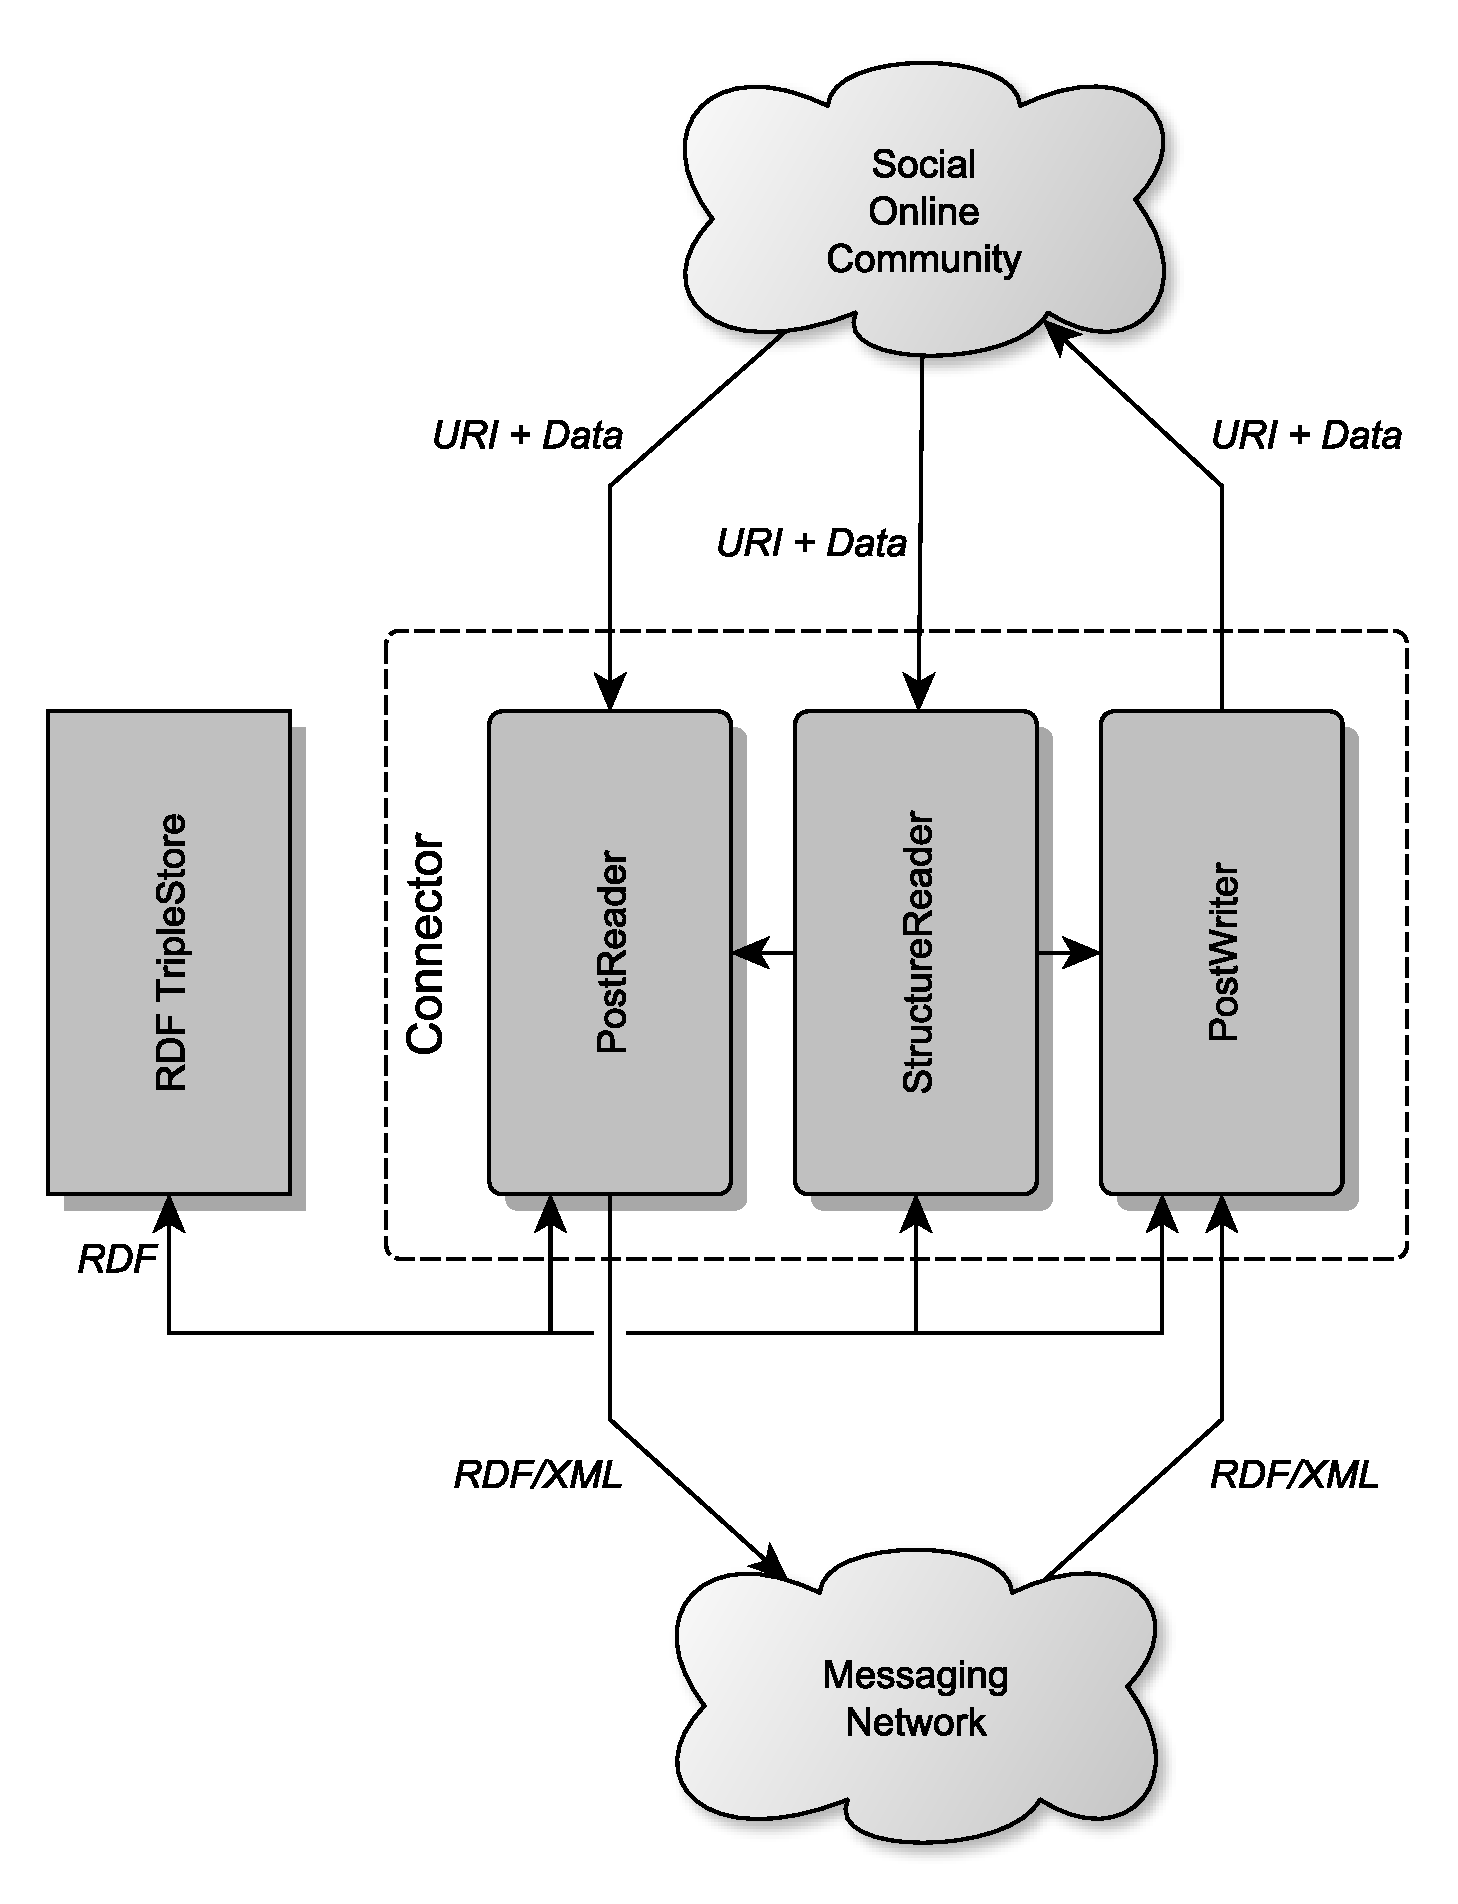
\includegraphics[
        width=0.5\textwidth,
        keepaspectratio=true]
    {assets/images/socc_connector_overview}
    \caption{Übersicht der Komponenten der SOCC}
    \label{fig:uebersicht_socc}
\end{figure}

Intern besteht ein Connector aus drei Komponenten die zum Einen für das Lesen (\emph{PostReader}) und Schreiben (\emph{PostWriter}) von Beiträgen verwendet werden, zum Andren aus einen \emph{StructureReader} der für das Auslesen der Struktur der Plattform verantwortlich ist. Eine genaue Beschreibung dieser Komponenten folgt in Abschnitt \ref{sec:design_eines_connectors}.

Jeder Connector hat Zugriff auf eine als \emph{Triplestore} bezeichnete Datenbank in der RDF-Triple gespeichert und mit SPARQL abgefragt werden können. Der Connector benutzt diesen Triplesore als Speicher in dem seine Konfigurationsdaten lagern, aber auch für zusätzliche Daten die er von Außerhalb benötigt. Er wird aber auch benutzt um Daten zu speichern, die während des Betriebes anfallen, da sie so irgendwann wieder verwendet werden können ohne sie erneut aus der von der Plattform laden zu müssen. Zum Beispiel die Daten über die Struktur der verwendeten Plattform, die sich selten ändert.

Die Beiträge werden dann zwischen den einzelnen Connectoren über ein Nachrichtennetzwerk auf der Basis von Apache Camel ausgetauscht. Die Beschreibung dieser als \emph{SOCC-Camel} bezeichneten Komponnente erfolgt in Abschnitt \ref{sec:socc_camel}.

% section datenformat (end)

\section{Konfiguration} % (fold)
\label{sec:konfiguration}

Damit ein Connector funktionieren kann, muss er von außen Informationen bekommen, welche er zum Betrieb braucht. Die sind zum Beispiel Informationen zu Benutzerkonten oder Parameter für die verwendete API. Da einige dieser Informationen nicht nur von einen Connector benutzt werden, ist es sinnvoll diese zusammen an einen Ort zu speichern und wiederverwenden zu können. Wofür der oben angesprochene Triplestore verwendet wird. Die wichtigsten Informationen für die Konfiguration der Connectoren stellen die Benutzerkonten dar. Sie enthalten unter anderem die Informationen, um Zugriff auf die Operationen der einzelnen APIs zu erhalten. Da die Benutzerkonten, wie später im Abschnitt \ref{sub:benutzerdaten} beschrieben, im FOAF-Format gespeichert werden, stellt es sich als Vorteil heraus die übrigen Informationen ebenfalls dort zu speichern und mit den schon vorhandenen zu verbinden. 

Aus diesem Grund wurde für Konfiguration eines Connectors die \emph{SOCC Connector Config Ontology} entwickelt. Diese Ontologie ist sehr einfach gehalten und baut auf schon vorhandenen Ontologien auf. Zusätzlich musste die SIOC-Ontologie so erweitert werden, dass die Integration von Authentifizierungs- und Autorisierungsinformationen möglich war. 

\subsection{SOCC Connector Config Ontologie} % (fold)
\label{sub:connector_config_ontologie}

Der Aufbau der SOCC Connector Config Ontologie (RDF-Präfix \texttt{ccfg:}) ist in der Abbildung \ref{fig:uebersicht_conector_cfg} zu sehen. Die Konfigurationsdaten für einen Connector werden dabei durch die Klasse \texttt{ccfg:ConnectorConfig} modelliert. Diese Klasse enthält dann die folgenden Eigenschaften für den Connector.

\begin{figure}[ht]
    \centering
    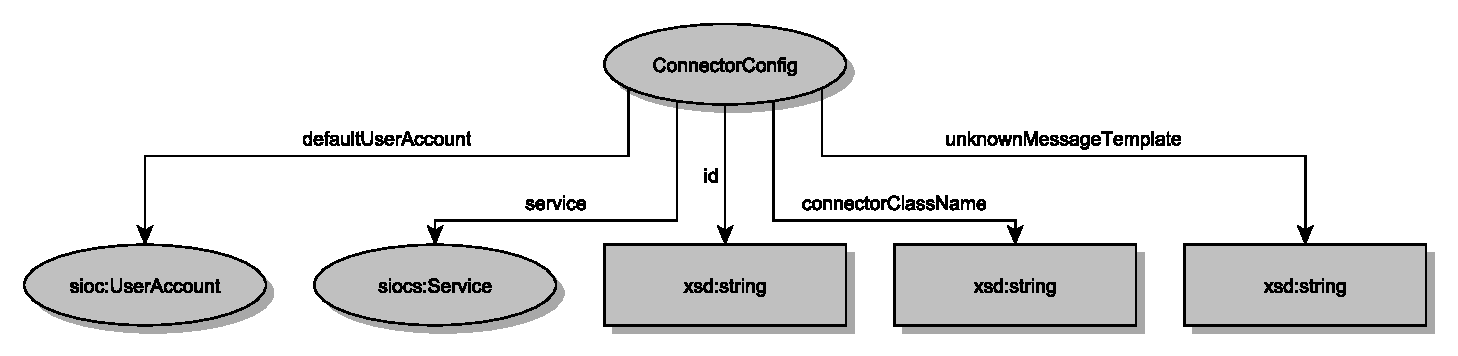
\includegraphics[
        width=\textwidth,
        keepaspectratio=true
    ]{assets/images/connector_config_ontology}
    \caption{Schema der SOCC Connector Config Ontology}
    \label{fig:uebersicht_conector_cfg}
\end{figure}

Jeder Connector erhält einen eindeutigen \texttt{ccfg:id} zugewiesen, um jeden Connector später eindeutig identifizieren zu können. Die Eigenschaft \texttt{ccfg:connectorClassName} beschreibt den vollständigen Java-Klassennamen des beschriebenen Connectors. Diese wird für das Laden der richtigen Implementierung benötigt. Manchmal kann es passieren, dass keine passendes Benutzerkonto zum Schreiben eins Beitrags gefunden werden kann. Dadurch es es wünschenswert solche Beiträte dahingegen zu verändern, dass eine Verweis auf den original Autor und vielleicht wo der Beitrag gemacht wurde vorhanden ist. Durch die Eigenschaft \texttt{ccfg:unknownMessageTemplate} kann eine Vorlage für das Aussehen des Verweises definiert werden. Innerhalb dieser Vorlage stehen einige Variablen in der Form \enquote{\texttt{\{varName\}}} zur Verfügung, wobei \enquote{varName} durch den Namen der entsprechenden Variable zu ersetzen ist. Welche Variablen alle vorhanden sind und mit welchen Werten diese ersetzt werden, ist in Tabelle \ref{tbl:unknown_message_template_vars} zu sehen. 

\begin{table}[ht]
    \caption{Variablennamen und Ersetzung innerhalb von \texttt{ccfg:unknownMessageTemplate} }
    \centering
    \begin{tabular}{l|l}
        \textbf{varName} & \textbf{Ersetzt durch} \\
        \hline
        \texttt{message} & Original Beitrag \\
        \texttt{sourceUri} & URI des original Beitrags \\
        \texttt{connectorId}  & ID des aktuellen Connectors \\
        \texttt{serviceName}  & Name des vom Connector verwendeten Service \\
        \texttt{creationDate} & Erstelldatum des Beitrags (falls bekannt) \\
        \texttt{authorName}   & Name des Autors (falls bekannt)          
    \end{tabular}
    \label{tbl:unknown_message_template_vars}
\end{table}

Für die Nutzung einiger APIs müssen zusätzlich bestimmte Parameter angegeben werden. Dies könnte zum Beispiel die genau Adresse des Dienstes sein. Hierzu wird auf das \emph{SIOC Services Modul} zurückgegriffen. Diese stellt eine Klasse \texttt{sioc:Service} zur Verfügung und über die Eigenschaft \texttt{ccfg:service} kann eine solche Servicebeschreibung einen Connector zugewiesen werden. Der genaue Aufbau eines solchen Services wird im Abschnitt \ref{sub:services} dargestellt. Die letzte Information für die Konfiguration eins Connectors ist eine Standardbenutzer (Im Folgenden Defaultuser genannt) und wird mit der Eigenschaft \texttt{ccfg:defaultUserAccount} festgelegt. Dieser Defaultuser erfüllt im Großen und Ganzen zwei Aufgaben. Als Erstes wird er für lesende Zugriffe der API auf die verwendete Plattform genutzt. Hierzu ist ein einzelnes Benutzerkonto vollkommen ausreichend, da nur die gelesenen Daten wichtig sind und nicht von welchen Konto sie kommen. Es sollte aber ein Konto mit weitreichenden Befugnissen sein, um möglichst viel Daten lesen zu können.Die zweite Aufgabe bezieht sich auf das stellvertretende Schreiben einzelner Benutzer. Nicht immer werden die dazu notwendigen Daten von den Benutzer zur Verfügung gestellt oder sind unbekannt. In diesem Fall wird der Defaultuser genutzt und der Inhalt des Beitrags in die Form der mit der Eigenschaft \texttt{\texttt{ccfg:unknownMessageTemplate}} festgelegten Vorlage konvertiert. 

% subsubsection connector_config_ontology (end)

\subsection{Services} % (fold)
\label{sub:services}

Wie eben schon beschrieben, existiert für SIOC ein Modul zur einfachen Modellierung von Diensten auf semantischer Ebene: Das SIOC Services Module (RDF-Präfix \texttt{siocs:}). Kernstück dieses Moduls ist die Klasse \texttt{siocs:Service}, wie auf Abbildung \ref{fig:uebersicht_sioc_services} zu sehen ist. Mit dieser Klasse kann durch eine Hand voll Eigenschaften ein Service beschrieben werden. Für diese Arbeit ist davon die wichtigste Eigenschaft \texttt{siocs:service\_endpoint}. Durch diese kann die Adresse festgelegt werden, unter dem ein Service erreichbar ist. Gerade bei Plattformen die nicht an eine feste Adresse (Foren, Blogs, $\dots$) gebunden sind, ist diese Angabe unerlässlich. Die Eigenschaften \texttt{siocs:has\_service} und \texttt{siocs:service\_of} sind ideal zur Verbindung von einzelnen \texttt{sioc:UserAccount}s mit einem Service. Diese Verbindung hilft dabei für das stellvertretende Schreiben von Beiträgen schnell die passenden Benutzerdaten zu finden. Ebenfalls nützlich ist \texttt{siocs:max\_results}. Manche Dienste erlauben es nur eine maximale Anzahl an Ergebnissen pro Aufruf zurückgeben zu lassen. Da sich diese Anzahl über die Zeit ändern kann ist es nicht sinnvoll diese fest im Programm festzulegen. Für SOCC weniger interessant aber der Vollständigkeit halber seien noch \texttt{siocs:service\_protocol} zum Angeben des verwendeten Übertragungsprotokolls REST, SOAP, $\dots$) und \texttt{siocs:service\_definition} mit dem auf eine weiterführende Definition verwiesen werden kann erwähnt. 

\begin{figure}[ht]
    \centering
    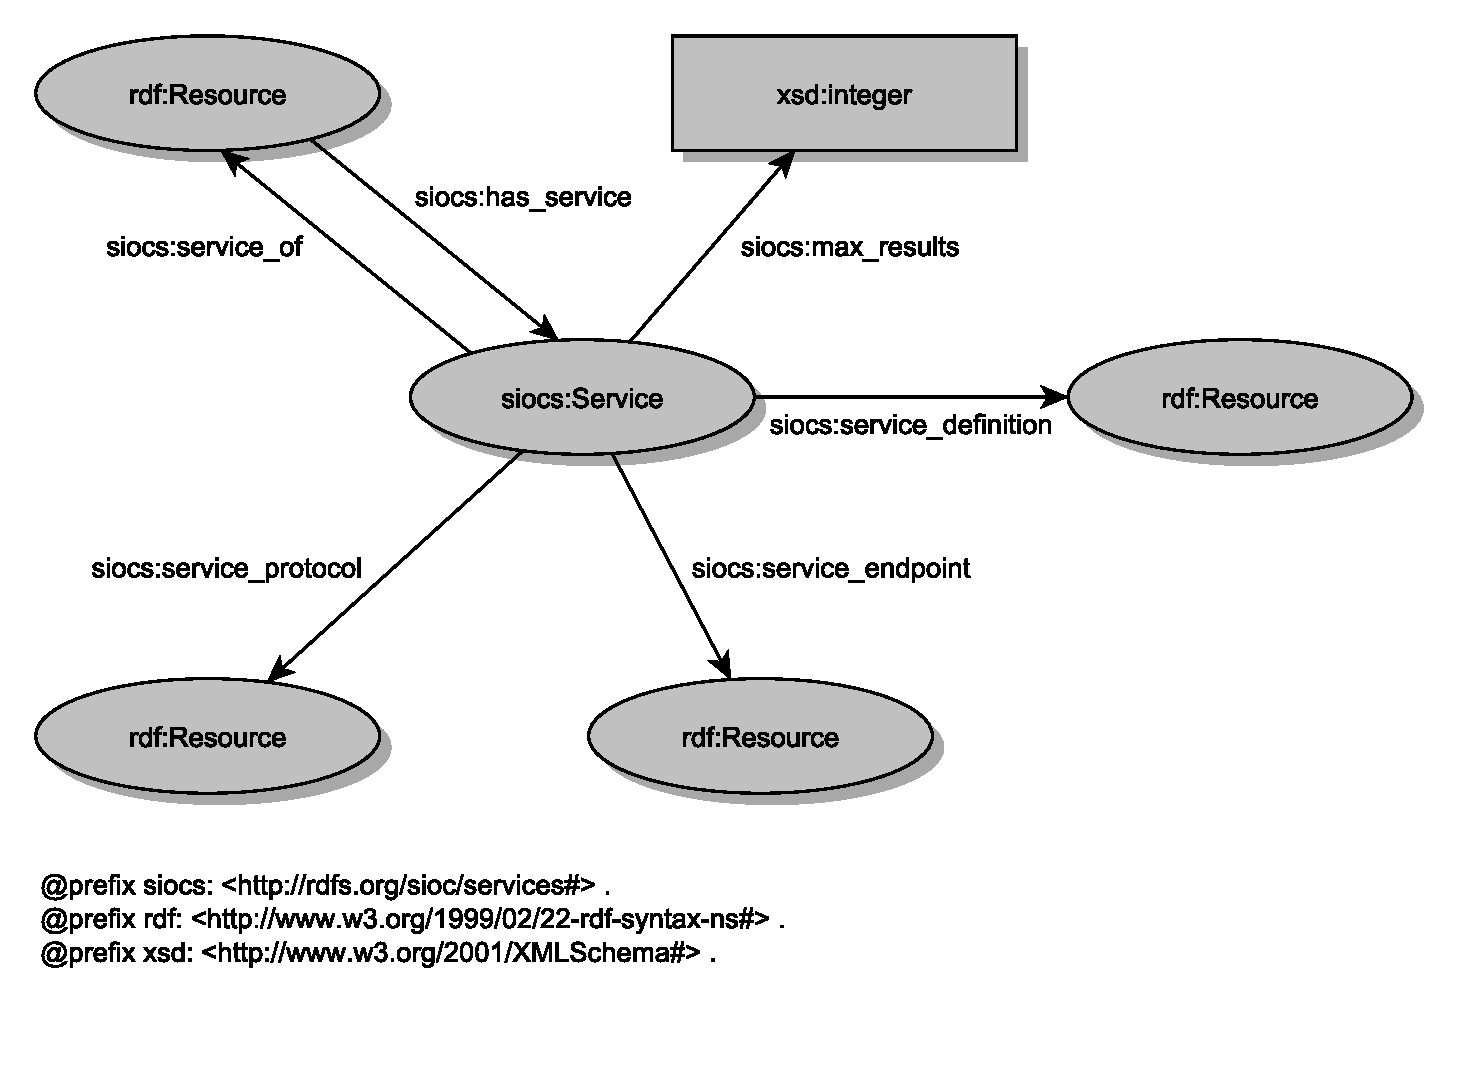
\includegraphics[
        width=\textwidth,
        keepaspectratio=true
    ]{assets/images/sioc_services_ontology}
    \caption{SIOC Services Module}
    \label{fig:uebersicht_sioc_services}
\end{figure}

% subsection services (end)

\subsection{Benutzerdaten} % (fold)
\label{sub:benutzerdaten}

Soll ein Beitrag eines Benutzers von Google+ nach Facebook synchronisiert werden und es so aussehen, als hat er diesen Beitrag selbst auf Facebook geschrieben, sind gute Kenntnisse über alle Benutzerkonten dieser einen Person notwendig. Als erstes muss die Existenz dieser Person dem System bekannt sein. Hierzu kann diese durch die Klasse \texttt{foaf:Person} aus der FOAF Ontologie dargestellt werden. Für ein einzelnes Benutzerkonto wurde in SIOC die Klasse \texttt{sioc:UserAccount} definiert. Da \texttt{sioc:UserAccount} eine Unterklasse von \texttt{OnlineAccount} aus FOAF ist, kann diese über die Eigenschaft \texttt{foaf:account} beziehungsweise \texttt{sioc:account\_of} mit einer Person verbunden werden. Ebenso ist es wichtig zu wissen zu welchen Plattform ein Benutzerkonto gehört. Deshalb wird der \texttt{sioc:UserAccount} mit einem Objekt der Klasse \texttt{siocs:Service} über die Eigenschaft \texttt{siocs:has\_service}/\texttt{siocs:service\_of} zusammengebracht. Diese Verbindung ist für manche APIs besonders bedeutend, da in dem Serviceobjekt relevante Daten für den Zugriff darauf enthalten sind. Nun kann es vorkommen, dass eine Person mehrere Benutzerkonten für private und geschäftliche Dinge besitzt. Um nicht private Beiträge auf Webseite A mit dem geschäftlichen Benutzerkonto auf Webseite B zu schreiben, muss ein Mapping zwischen den verschiedenen Benutzerkonten festgelegt werden. Dieses Mapping kann über ein in der \enquote{\nameref{sec:anhang_socc_connector_config_ontologie}} definierte Eigenschaft \texttt{ccfg:mapped\_to} realisiert werden. Diese Eigenschaft ist symmetrisch, also falls Benutzerkonto A mit Benutzerkonto B über \texttt{mapped\_to} verbunden ist, dann gilt dies ebenfalls für B mit A. Abbildung \ref{fig:usermanagement} zeigt den Zusammenhang zwischen der Klasse \texttt{foaf:Person}, \texttt{sioc:UserAccount} und \texttt{siocs:Service} sowie der Eigenschaft \texttt{ccfg:mapped\_to} noch einmal graphisch an einem Beispiel.

\begin{figure}[ht]
    \centering
    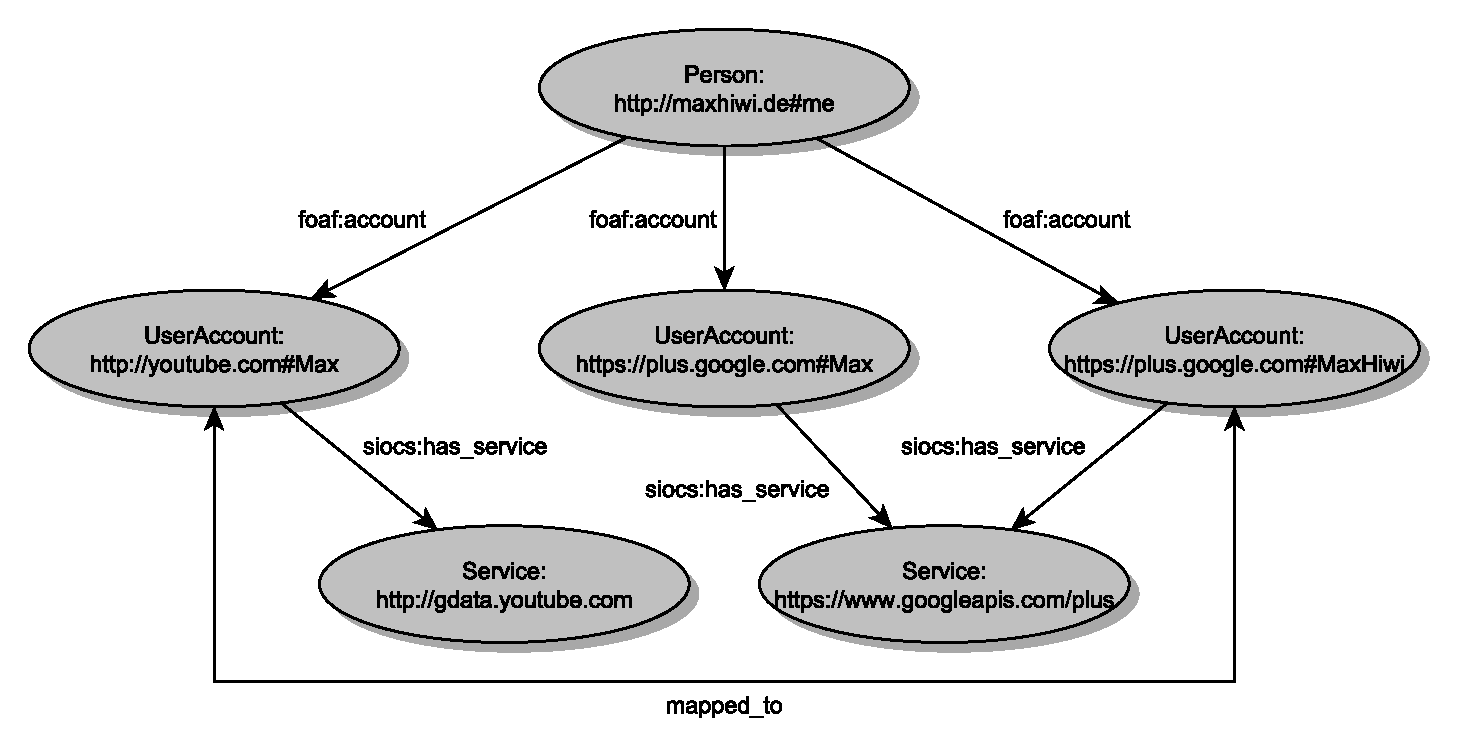
\includegraphics[
        width=\textwidth,
        keepaspectratio=true,]
    {assets/images/usermanagement}
    \caption{Zusammenhang von Person, UserAccount und Service. Die inversen Eigenschaften \texttt{sioc:account\_of} und \texttt{siocs:service\_of} wurden zu einer besseren Übersicht weggelassen}
    \label{fig:usermanagement}
\end{figure}

% subsubsection benutzerdaten (end)

\subsection{Authentifizierung} % (fold)
\label{sub:authentifizierung}

Die Ontologien FOAF und SIOC sind hervorragend für die Abbildung von sozialen Netzwerken und Diskussionen, jedoch ist es mit ihnen nicht möglich Daten zur Authentifizierung (Feststellen ob jemand der ist, den er vorgibt zu sein). Wegen dem Schutz der Privatsphäre ist dies verständlich, jedoch um stellvertretend für einen Benutzer Beiträge zu schreiben, ist es wichtig Zugriff auf diese Daten zuhaben und sie einem Benutzerkonto zuordnen zu können. Zuerst muss dazu aber festgestellt werden, welche verschiedenen Mechanismen es zum Anmelden ein solches Konto existieren.

\begin{description}
    \item[Username/Passwort] ist wohl eine der ersten und häufigsten Mechanismen, um den Zugriff sensibler Daten vor Dritten zu schützen. Das in Abschnitt \ref{sub:moodle_connector} beschriebene LMS Moodle, setzt zum Beispiel den Username und Password eines angemeldeten Benutzers zu Authentifizierung ein.
    
    \item[OAuth]\footnote{OAuth Webseite: \url{http://oauth.net/}} stellt heutzutage den Standard der verwendeten Authentifizierungsmechanismen für hauptsächlich webbasierte API dar. Benutzer können so temporär Programmen den Zugriff auf ihre Daten erlauben und später wieder verbieten. Der aktuelle Standard stellt OAuth 2.0 dar und wird in dieser Version von den größten Seitenbetreibern wie Google, Facebook oder Microsoft eingesetzt\footnote{OAuth Versionen im Einsatz: \url{http://en.wikipedia.org/wiki/OAuth\#List\_of\_OAuth\_service\_providers}}. Insgesamt sind für die Nutzung von OAuth vier Parameter wichtig. Für das Programm, dass Zugriff erhalten möchte sind die Parameter \emph{client\_id} und \emph{client\_secret} (Siehe \cite{rfc6749}[S.\,8]). Sie weisen das Programm als autorisiert für die Benutzung der Schnittstelle aus. Soll nun beim Aufrufer einer von OAuth geschützten Funktion belegt werden ist ein sogenannter Accesstoken nötig (Siehe \cite{rfc6749}[S.\,9]). Da dieser Accesstoken in der Regel nur eine bestimmte Zeit gültig ist, wird je nach Implementierung des Standards noch ein Refreshtoken mitgeliefert. Mit diesem Refreshtoken ist das Programm in der Lage ohne Zutun des Benutzers einen abgelaufen Accesstoken wieder zu aktivieren. Dies kann beliebig oft wiederholt werden, bis der Benutzer beide Token für ungültig erklärt.
    \todo[inline]{vll. noch OAuth 1.0(a) einbauen}
    
    \item[API Schlüssel] sind eine dritte Möglichkeit Programmen Zugriff auf eine API zu gewähren. Der API Schlüssel entspricht ungefähr einer Kombination von client\_id und client\_secret von OAuth. Dieser Schlüssel schaltet in der Regel nicht den Zugriff auf persönliche Daten von Benutzer frei. Hier ist noch ein weiterer Mechanismus wie die Verwendung von einem Usernamen und Passwort nötig. Die in Abschnitt \ref{sub:youtube_connector}  beschriebene Google Youtube API hierzu ein gutes Beispiel.
\end{description}

\begin{figure}[ht]
    \centering
    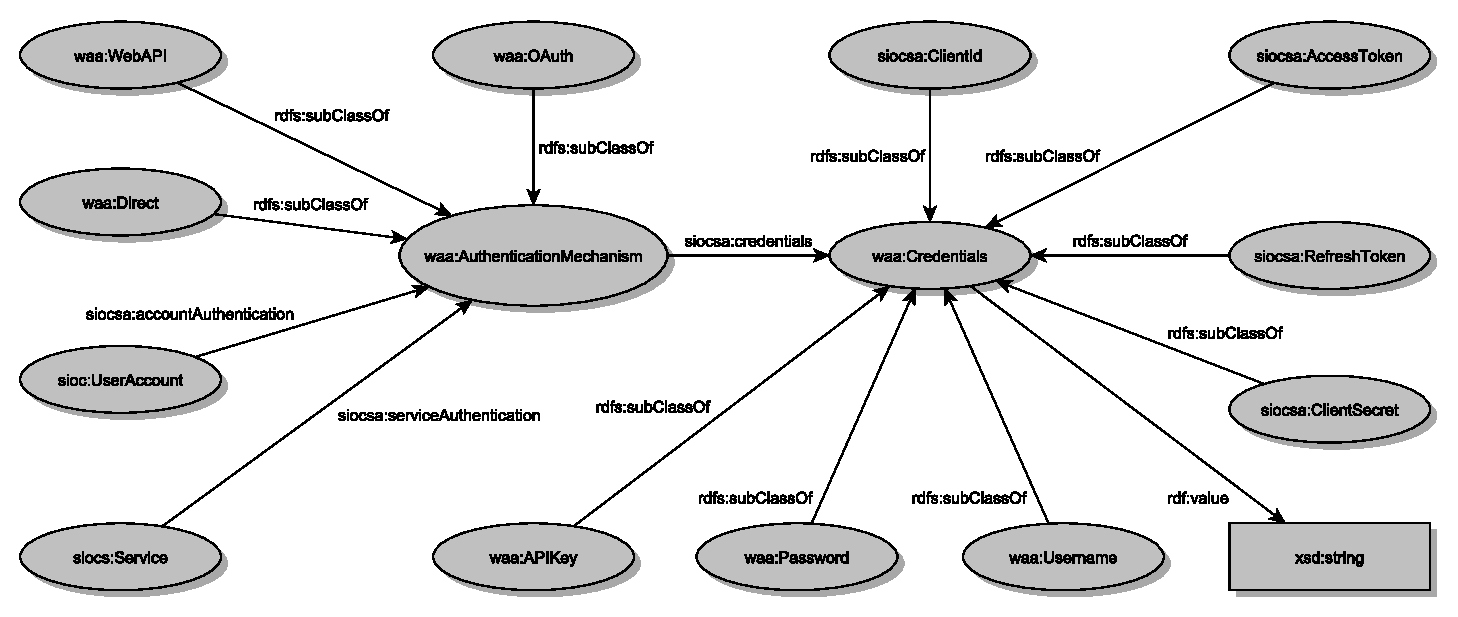
\includegraphics[
        width=\textwidth,
        keepaspectratio=true]
    {assets/images/sioc_services_authentication}
    \caption{SIOC Services Authentication Ontology}
    \label{fig:uebersicht_sioc_services_authentication}
\end{figure}

Neben diesen drei Mechanismen wäre noch der Vollständigkeit halber die HTTP-Authentifizierung zu nennen. Hierbei handelt es ich um eine Form des Username/Passwort Verfahrens, welches auf dem HTTP Protokoll aufsetzt. Für einfachen Webseiten ist dies ein unkomplizierte Art die Datei vor fremden Zugriffen zu schützten. Für aktuelle öffentliche APIs ist diese Form der Authentifizierung nicht mehr Stand der Technik.

Die Suche nach einer bestehen Ontologie, welche zusammen mit SIOC verwendet werden könnte, gestaltete sich als sehr schwierig. Ein Großteil der Ontologien in diese Richtung befasst sich eher mit dem Thema der Autorisierung wie zum Beispiel die \emph{Web Access Control List} \cite{Hollenbach2009} mit Zugriffssteuerungsliste. Eine Ausnahme stellt die \emph{Authentication Ontology}\footnote{Authentication Ontology: \url{http://omnivoke.kmi.open.ac.uk/authentication/}} (RDF-Prefix \texttt{waa:}) des \emph{OmniVoke}\footnote{OmniVoke: \url{http://omnivoke.kmi.open.ac.uk/framework/}} Frameworks dar. Die Art der Authentifizierung wird darin durch die Klasse \texttt{waa:AuthenticationMechanism} modelliert. Unterklassen für die wichtigsten Mechanismen wie \texttt{waa:OAuth}, \texttt{waa:WebAPI}s und Username/Password (dort \texttt{waa:Direct} genannt) sind vorhanden. Jedem AuthenticationMechanism Objekt können dann sogenannte \texttt{waa:Credentials} (engl. für Anmeldedaten) angehängt werden.

Das einzige Manko an dieser Ontologie war das Fehlen von Credentials für OAuth in der Version 2.0. Im einzelnen waren dies Klassen für clien\_id, client\_secret sowie für Access- und Refreshtoken. Um auch diese OAuth Version unterstützen zu können, wurden hierfür die Klassen ClientId, ClientSecret, AccessToken und RefreshToken als Unterklassen von Credentials abgeleitet. Als Letztes musste noch eine Verbindung zwischen Authentication Ontology und SIOC hergestellt werden. Zum Einen war eine Erweiterung der Klasse \texttt{sioc:UserAccount} notwendig, so dass die Anmeldedaten der Benutzer zur Verfügung standen. Zum Anderen werden Daten wie ein API-Schlüssel von einem Service benötigt, die von denen der Benutzer unabhängig sind. Für die Klasse \texttt{sioc:UserAccount} wurde die Eigenschaft \texttt{siocsa:accountAuthentication} geschaffen. Diese erwartet als Subjekt einen \texttt{sioc:UserAccount} und als Objekt ein AuthenticationMechanism, welcher dann die Credentials enthält. Für die Klasse \texttt{sioc:Service} existiert das Äquivalent \texttt{siocsa:serviceAuthentication}. 

Diese Erweiterungen und die übernommenen Teile der Authentication Ontology wurden danach im \emph{SIOC Services Authentication Module} (RDF-Präfix \emph{siocsa:}) zusammengefasst. Graphisch ist sie in Abbildung \ref{fig:uebersicht_sioc_services_authentication} und im Anhang \ref{sec:anhang_sioc_services_authentication_module} als OWL Schema zu sehen. 

% subsection authorization (end)

\subsection{Autorisierung} % (fold)
\label{sub:autorisierung}
%% korrigiert am 2013-09-26 20:10

Da für viele Menschen im Internet ihre Privatsphäre wichtig ist und sie nicht wollen, ist es wichtig von ihnen die Erlaubnis einzuholen, um ihr Beiträge zu lesen und weiterzuleiten. Ein verbreitetes Mittel für eine solche Zugriffssteuerung sind Access Control Lists (ACL) (engl. für Zugriffsteuerungsliste). Mit ihnen wird geregelt wer bestimmte Operationen auf eine Ressource durchführen darf. Für den Einsatz in dieser Arbeit wurde die Basic Access Control Ontologie (siehe \cite{Hollenbach2009,wiki:wacl})(RDF-Präfix \texttt{acl:}) ausgewählt (Im Folgenden nur als ACL bezeichnet). Da sie Teilweise auf FOAF aufbaut und so ließ sie sich sehr einfach in das bestehende System integrieren.

\begin{figure}[ht]
    \centering
    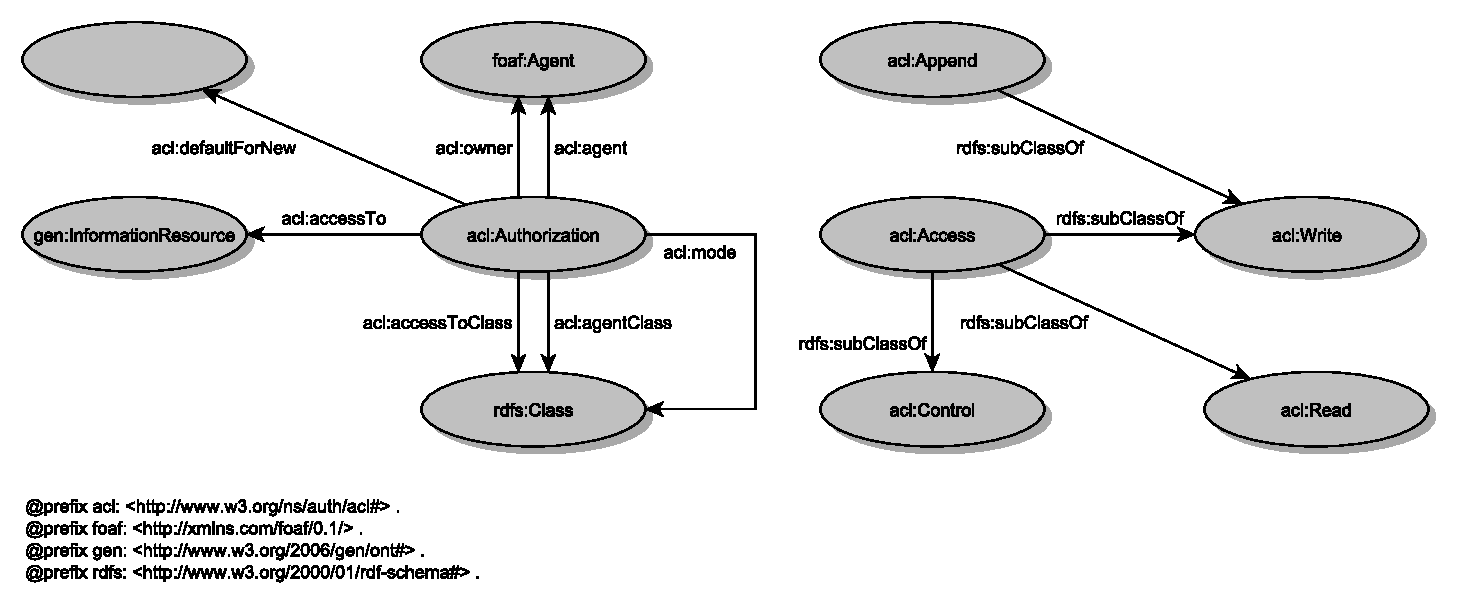
\includegraphics[
        width=\textwidth,
        keepaspectratio=true]
        {assets/images/w3c_web_acl}
    \caption{Basic Access Control Ontologie}
    \label{fig:w3c_web_acl}
\end{figure}


Zugriffsrechte für Ressourcen werden in dieser ACL mit der Klasse \texttt{acl:Access} modelliert. Von dieser Klasse werden einzelne Rechte wie \texttt{acl:Read} für das Lesen und \texttt{acl:Write} für das Schreiben abgeleitet. Nebenbei existieren noch Ableitungen \texttt{acl:Control} zum Ausführen und \texttt{acl:Append} zum Anfügen von Daten an die Ressource.

Die Verbindung von einen Zugriffsrecht mit eine Ressource wird über die Klasse \texttt{acl:Authorization} erreicht. Der Besitzer dieser Autorisierung wird durch die Eigenschaft \texttt{alc:owner} festgelegt und gehört zur Klasse \texttt{foaf:Agent} beziehungsweise der davon abgeleiteten Klasse \texttt{foaf:Person}. Mittels der Eigenschaft \texttt{acl:agent} wird festgelegt für welche Person/Agenten diese Autorisierung gilt. Das selbe wird auch über die Eigenschaft \texttt{acl:agentClass} festgelegt, wobei hier eine abstrakte Klasse statt eine Instanz davon gemeint ist. Soll zum Beispiel der öffentlicher Zugriff für eine Ressource definiert werden, wird bei \texttt{acl:agentClass} die Klasse \texttt{foaf:Agent} eingesetzt \cite[\enquote{Public Access}]{wiki:wacl}. Dies besagt, dass alle Agenten auf diese Ressource zugreifen können. Innerhalb von SOCC werden Ressourcen verarbeiten, die öffentlich zugänglich sind. Welches Recht für eine Ressource eingeräumt wird, wird über die Eigenschaft \texttt{acl:mode} festgelegt. Erlaubt ist hier die Angabe jeder beliebigen Klasse, SOCC testet aber nur ob das Recht \texttt{acl:Read} zum Lesen oder \texttt{acl:Write} zum Schreiben von Beiträgen eingeräumt wurde. Auf welche Ressource  sich letztendlich eine Autorisierung bezieht, wird über die Eigenschaft \texttt{acl:accessTo} geregelt. Die Angabe von \enquote{http://www.facebook.com} würde sich für SOCC zum Beispiel auf alle Beiträge des Besitzers auf Facebook beziehen, \enquote{https://canvas.instructure.com/courses/798152} dahingegen nur auf alle Beiträge innerhalb eines Canvas Kurses mit der ID \enquote{798152}. Für einen Zugriff auf alle Beiträge prüft SOCC ob die Eigenschaft \texttt{acl:accessToClass} auf die Klasse \texttt{sioc:Post} verweist. So müsste nicht jede einzelne Webseite angegeben werden, wenn man ein generelles Zugriffsrecht einräumt.

Das Listing \ref{lst:acl_beispiel} zeigt ein Beispiel, wie eine Autorisierung mit der ACL aussehen könnte. Der Besitzer dieser Autorisierung mit der URI \texttt{http:/example.org\#john} wird in Zeile 6 beschrieben. Er erlaubt damit SOCC einen öffentlichen (Zeile 7), lesenden (Zeile 9) Zugriff auf all seine geschrieben Beiträge (Zeile 8).

\begin{lstlisting}[
    caption={ACL Beispiel}\label{lst:acl_beispiel},
    captionpos=t]
@prefix sioc: <http://rdfs.org/sioc/ns#> .
@prefix foaf: <http://xmlns.com/foaf/0.1/>
@prefix acl: <http://www.w3.org/ns/auth/acl#> .

[] a acl:Authorization ;
    acl:owner <http:/example.org#john> ;
    acl:agentClass foaf:Agent ;
    acl:accessToClass sioc:Post ;
    acl:mode acl:Read .
\end{lstlisting}

% subsection autorisierung (end)

% section konfiguration (end)

\section{Design eines Connectors} % (fold)
\label{sec:design_eines_connectors}

\begin{wrapfigure}{r}{8cm}
    \centering
    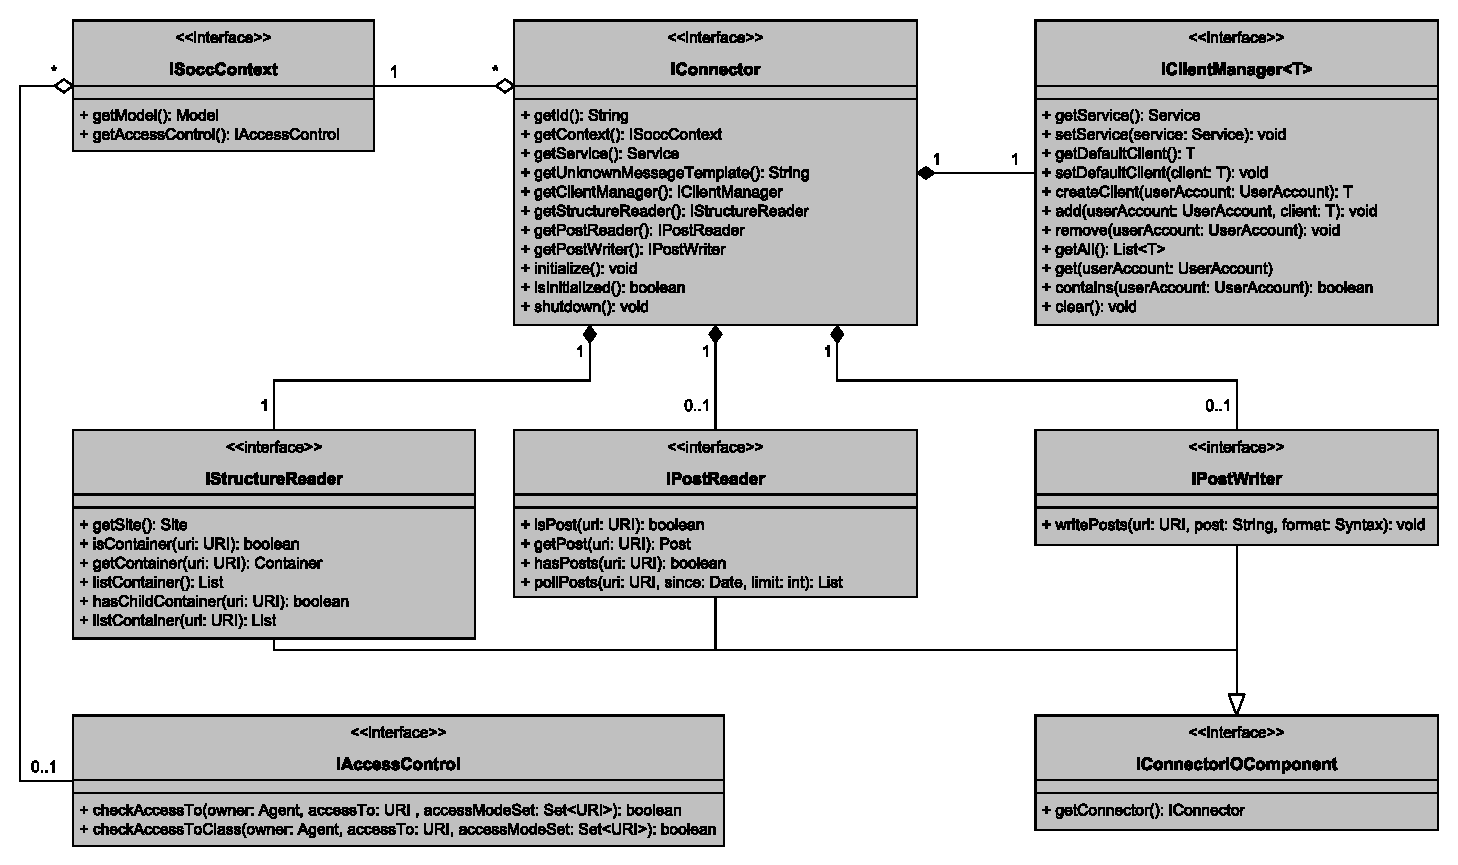
\includegraphics[
        width=8cm,
        keepaspectratio=true,
        clip=true,
        trim= 246 258 259 8]
    {assets/images/socc_uml_classdiagram}
    \caption{PostReader}
    \label{fig:uml_connector_interface}
\end{wrapfigure}

Die rechte Abbildung \ref{fig:uml_connector_interface} zeigt die Schnittstelle \texttt{IConnector} gegen die ein Connector implementiert werden muss. Sie bietet Zugriff auf die Eigenschaften die mit der Klasse ConnectorConfig für die Konfiguration eines Connectors im Triplestore bereitgestellt werden. Diese Schnittstelle definiert Methoden, um auf die einzelnen Komponenten zum Lesen der Seitenstruktur mit dem StructureReader sowie zum Lesen und Schreiben von Beiträgen mit PostReader und PostWriter zuzugreifen. Zuzüglich werden noch Methoden für den Zugriff Hilfskomponenten wie den \emph{SOCC Context}, \emph{AccessControl} und \emph{ClientManger} bereitgestellt. Das UML Klassendiagramm in Abbildung \ref{fig:connector_uml_classdiagram} zeigt die Beziehung zwischen den Connector und den Komponenten aus dem er besteht, welche in den folgenden Unterabschnitten noch weiter erklärt werden.

Für den Lebenszyklus eines Connectors sind noch die Methoden \texttt{initialize()} und \texttt{shutdown()} wichtig. Nach dem Erzeugen eines Connectors muss die Methode \texttt{initialize()} aufgerufen, um noch mögliche Vorarbeiten durchzuführen bevor der Connector genutzt werden kann. Ob eine Connector schon initialisiert wurde, kann mit der Methode \texttt{isInitialized()} überprüft werden. Bevor eine Connector gelöscht werden soll, sollte nicht die Methode \texttt{shutdown()} aufgerufen werden. Sie dient dazu ob verwendete Ressourcen wieder freizugeben.

\begin{minipage}{\textwidth}
    \centering
    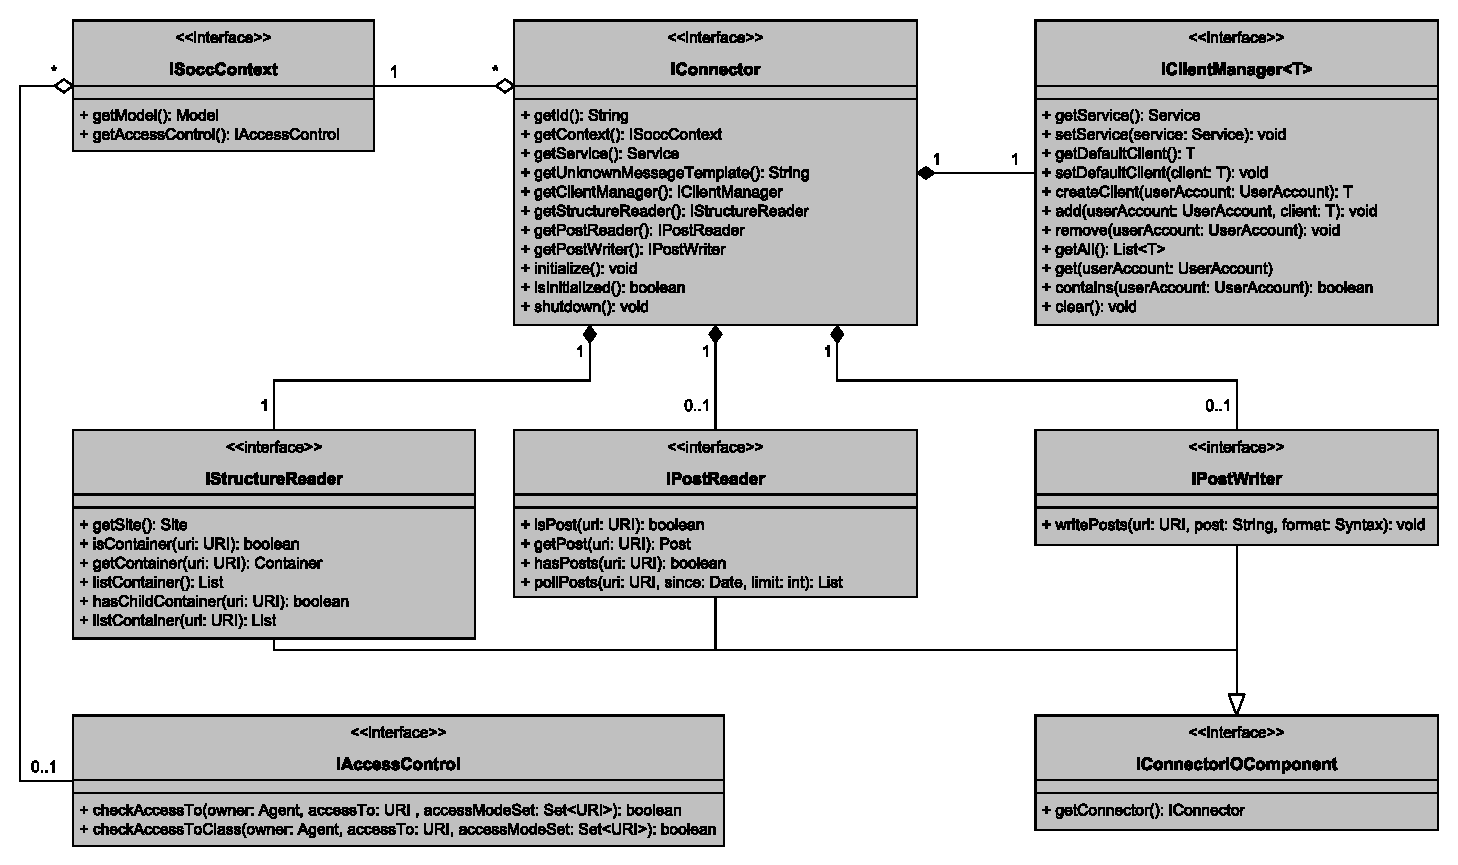
\includegraphics[
        scale=0.95,
        keepaspectratio=true,
        angle=90]
    {assets/images/socc_uml_classdiagram}
    \captionof{figure}{UML Klassendiagramm eines Connectors}
    \label{fig:connector_uml_classdiagram}
\end{minipage}

% subsection design_eines_connectors (end)

\subsection{SOCC Context} % (fold)
\label{sub:socc_context}
%% korrigiert am 2013-09-26 20:35

\begin{wrapfigure}{r}{6cm}
    \centering
    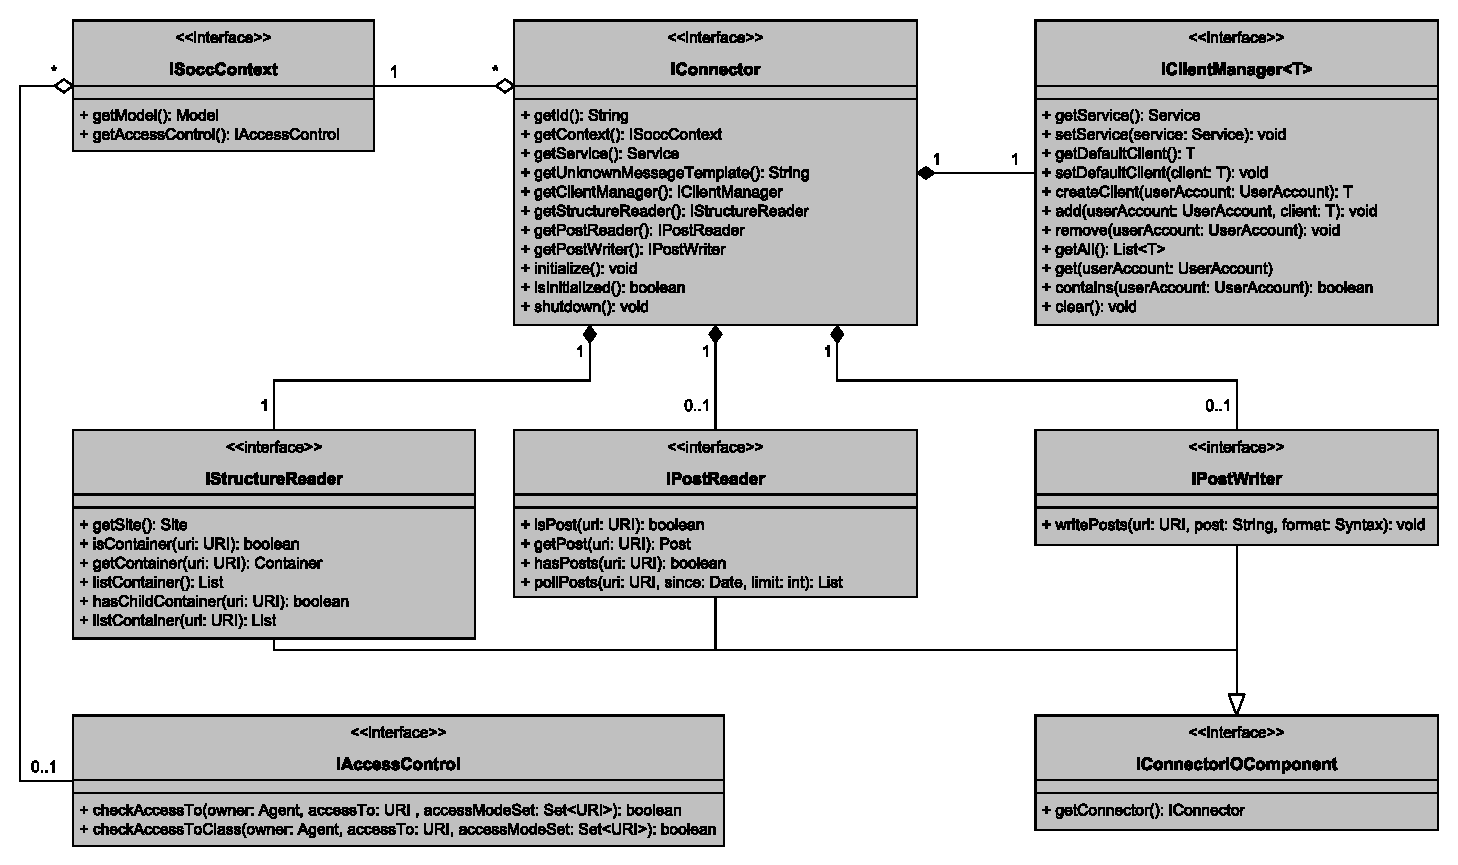
\includegraphics[
        width=6cm,
        keepaspectratio=true,
        clip=true,
        trim= 35 340 520 9]
    {assets/images/socc_uml_classdiagram}
    \caption{SOCC Context}
    \label{fig:uml_socc_context}
\end{wrapfigure}

Der SOCC Context eines Connectors, beschreibt die Umgebung die er zum Arbeiten braucht. Über ihn bekommt der Connector Zugriff auf den sich außerhalb befindlichen Triplestore, der durch die Klasse \texttt{Model} der RDF2Go Bibliothek abstrahiert wird (Siehe Abschnitt \ref{sec:verwendete_bibliotheken_und_programme}). In ihm befinden sich alle Daten die der Connector für seinen Betrieb benötigt und benutzt ihn gleichzeitig als Lagerplatz für welche die während des Betriebs gespeichert werden müssen. Eine Referenz auf dieses Triplestore erhält der Connector über den Aufruf der Funktion \texttt{getModel()}. Durch die Methode \texttt{getAccessControl()} kann der Connector über die im folgenden Abschnitt beschriebene AccessControl Schnittstelle auf die Information für die Zugriffssteuerung zugreifen. 

% subsubsection socc_context (end)

\subsection{AccessControl} % (fold)
\label{sub:accesscontrol}
%% korrigiert am 2013-09-26 20:38

\begin{wrapfigure}{r}{12cm}
    \centering
    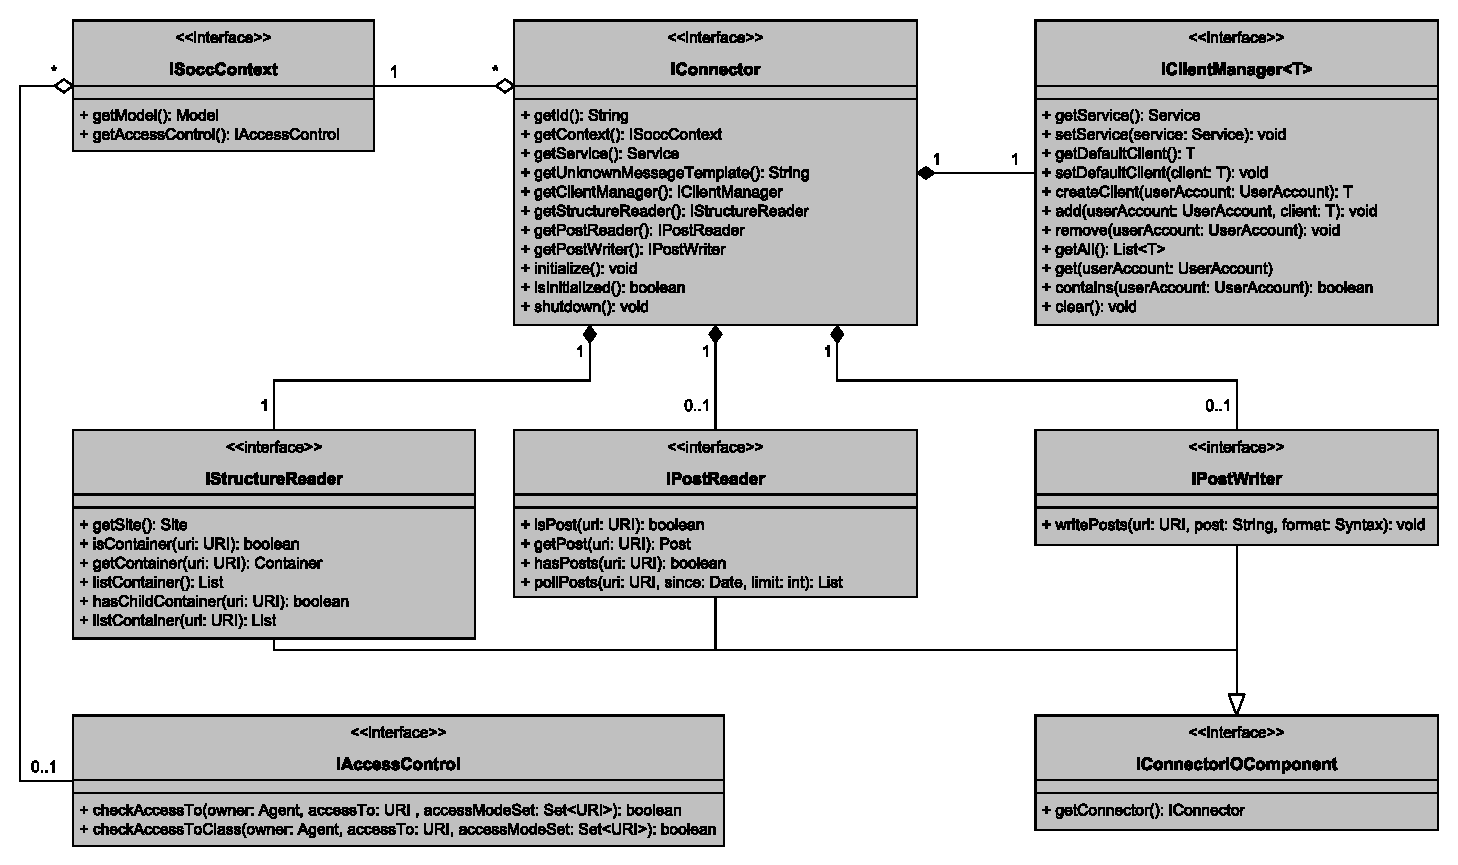
\includegraphics[
        width=12cm,
        keepaspectratio=true,
        clip=true,
        trim= 35 8 350 340]
    {assets/images/socc_uml_classdiagram}
    \caption{AccessControl}
    \label{fig:uml_accesscontrol}
\end{wrapfigure}

Die AccessControl Schnittstelle ist sehr einfach gehalten und dient für den Zugriff auf die in Abschnitt \ref{sub:autorisierung} beschriebenen ACL Information. Die Methode \texttt{checkAccessTo(\dots)} prüft, ob der Zugriff auf eine Ressource mit allen übergebenen Rechten erlaubt ist. Die andere Methode \texttt{checkAccessToClass} ist zur Überprüfung, ob die Rechte für den Zugriff auf eine komplette Klasse von Ressourcen vorhanden sind. 

% subsubsection accesscontrol (end)

\subsection{ClientManager} % (fold)
\label{sub:clientmanager}
%% korrigiert am 2013-09-26 20:50

\begin{wrapfigure}{r}{7cm}
    \centering
    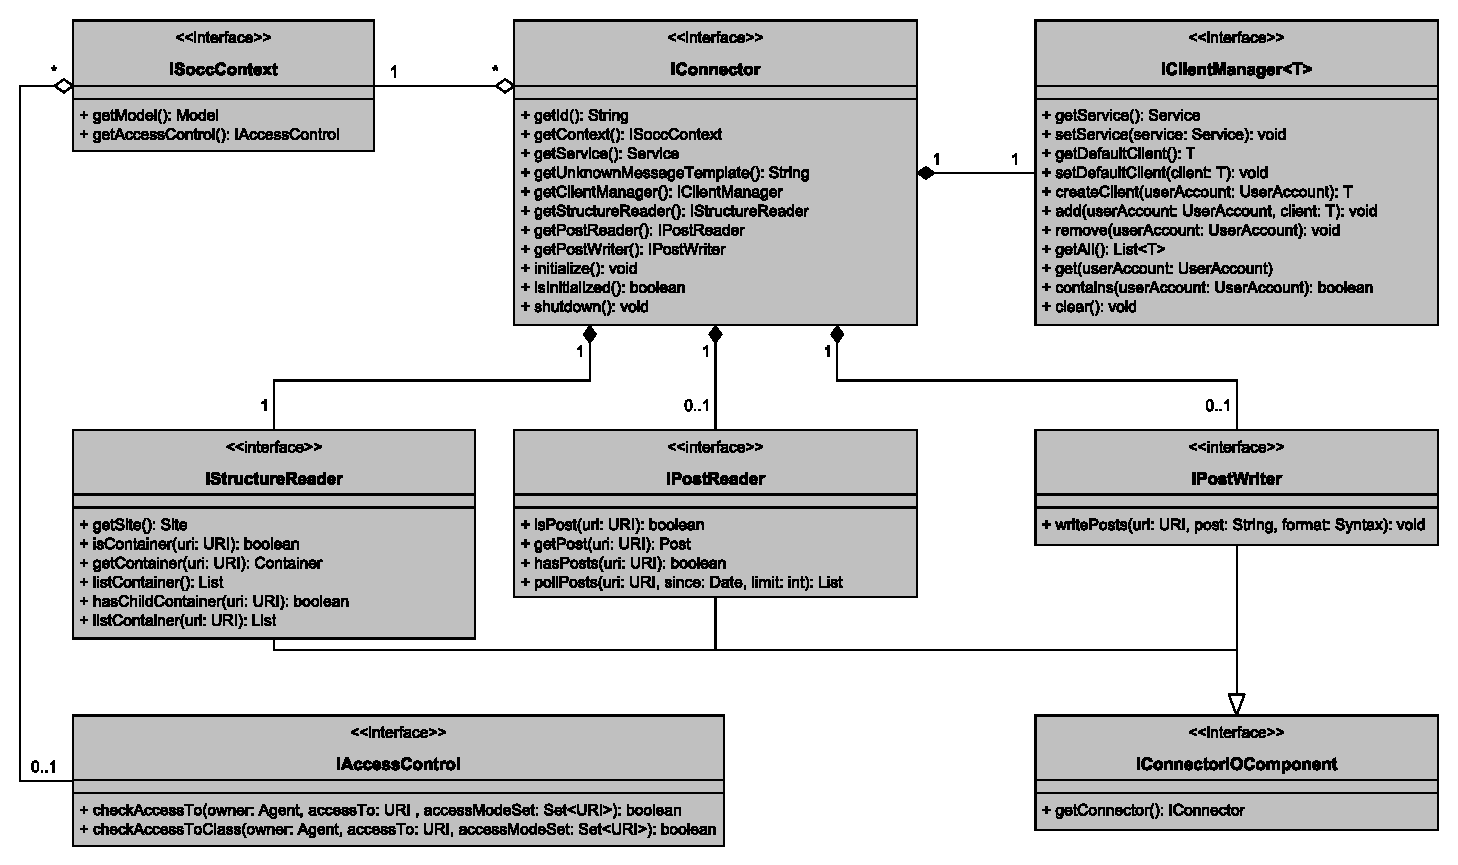
\includegraphics[
        width=7cm,
        keepaspectratio=true,
        clip=true,
        trim= 497 257 9 9]
    {assets/images/socc_uml_classdiagram}
    \caption{ClientManager}
    \label{fig:uml_clientmanager}
\end{wrapfigure}

Der Zugriff auf eine API innerhalb des Programms erfolgt in der Regel über ein spezielles Clientobjekt (kurz Client). Dieser Client erlaubt es mit den Anmeldedaten für ein Benutzerkonto auf die Funktionen der API über verschiedene Methoden zu zugreifen. Da ein Client immer nur mit einem Benutzerkonto verknüpft ist und von diesen eine große Anzahl verwaltet werden müssen, enthält jeder Connector einen eigen ClientManager für diese Aufgaben. Der interne Aufbau eines Client ist dabei stark von der verwendeten API abhängig und wird als generischer Parameter der Klasse beim erzeugen eines Objekts übergeben. Für alle vom Benutzer unabhängigen Daten erhält der ClientManager ein, wie Abschnitt \ref{sub:services} beschriebenes, Objekt der Klasse Service, dass zum Beispiel die Basis-URI für die API enthält. Das Erzeugen eines neuen Clients erfolgt dann durch den Aufruf der Methode \texttt{createClient(\dots)}. Als Parameter wird er ein Benutzerkonto, in Form eines SIOC UserAccounts, übergeben. Sind alle erforderlichen Authentifizierungsinformation aus Abschnitt \ref{sub:authentifizierung} vorhanden, wird ein neuer Client erzeugt und zurück an den Aufrufer gegeben. Dieser Client wird aber dadurch nicht automatisch vom ClientManager verwaltet. Hierzu muss der im vorherigen Schritt erzeugte Client durch die Übergabe an \texttt{add(userAccount: UserAccount, client: T )} dauerhaft mit den angegeben UserAccount verknüpft und intern gespeichert werden. In der aktuellen Implementierung ist es wichtig, dass die Eigenschaften \texttt{accountName} und \texttt{accountServiceHomepage} des UserAccount Objekts gesetzt sind. Aus diesen wird ein eindeutiger Schlüssel generiert, der zur Zuordnung von UserAccount und Client innerhalb des ClientManagers dient. Des weiteren stehen noch Methoden \texttt{remove(userAccount: UserAccount)} zum Entfernen und \texttt{get(userAccount: UserAccount)} zum Holen von Clients, sowie \texttt{contains(userAccount: UserAccount)} für Tests, ob ein Client zu einem UserAccount existiert, zur Verfügung. Sollen zum Beispiel am Ende der Laufzeit des Programms alle erzeugten Clients auf einmal abgemeldet und gelöscht werden, kann dies über die Methode \texttt{clear()} erfolgen. Der ClientManager verwaltet ebenfalls den Client für den in Abschnitt \ref{sub:connector_config_ontologie} angesprochenen Defaultuser. Dieser Defaultclient genannte Client kann über die Methode  \texttt{setDefaultClient(client: T)} gesetzt und durch \texttt{getDefaultClient()} jederzeit wieder abgerufen werden. 

% subsubsection clientmanager (end)

\subsection{StructureReader} % (fold)
\label{sub:structurereader}
%% korrigiert am 2013-09-26 21:07

\begin{wrapfigure}[11]{r}{9cm}
    \centering
    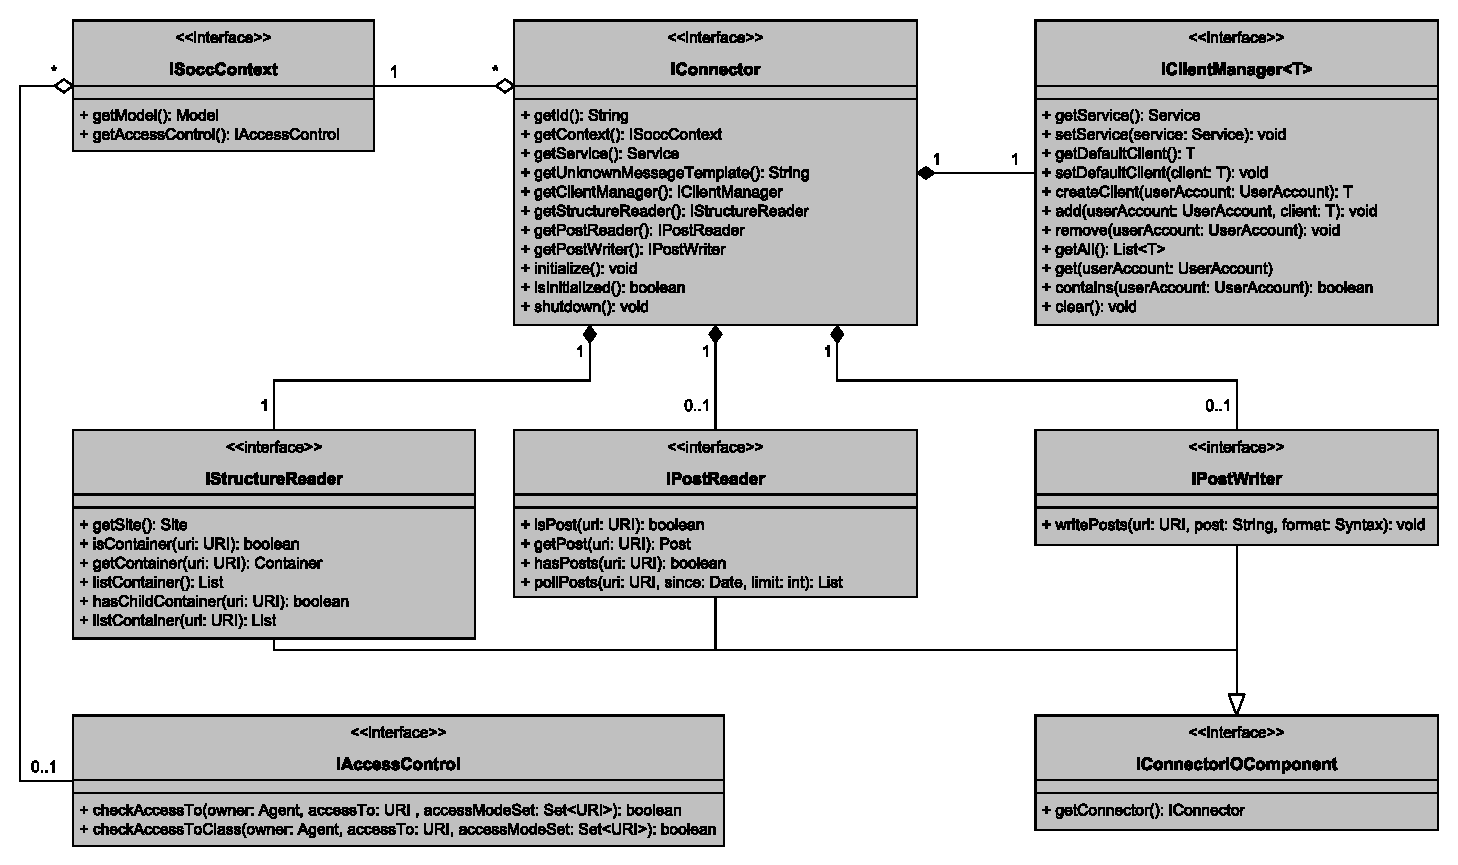
\includegraphics[
        width=9cm,
        keepaspectratio=true,
        clip=true,
        trim= 20 109 456 206]
    {assets/images/socc_uml_classdiagram}
    \caption{StructurReader}
    \label{fig:uml_structure_reader}
\end{wrapfigure}
Um auf Informationen über die Struktur von Foren, sozialen Online-Netzwerken und so weiter im SIOC-Format zugreifen zu können, implementiert jeder Connector dazu einen StructureReader. Die Struktur lässt sich, wie im Abschnitt \ref{ssub:semantically_interlinked_online_communities} vorgestellt, durch die SIOC Klassen \emph{Site} und \emph{Container} (sowie Unterklassen davon) beschrieben. Für den Zugriff auf diese Struktur, enthält der StructureReader mehrere Methoden die in der UML Klasse rechts in Abbildung \ref{fig:uml_structure_reader}) zu sehen sind. \wrapfill

\begin{description}
    \item[\texttt{getSite()}] ist eine Methode, welche die Beschreibung einer Seite (Forum, Blog, soziales Online-Netzwerk) als Objekt der SIOC-Klasse \texttt{Site} zurücklieft. Dieses wird relativ häufig gebraucht um die Zugehörigkeit anderer Objekte durch einen Verweis zu dieser Seite zu verdeutlichen. Dies kann bei einigen APIs nützlich sein, da dort manchmal keine Information zum Ursprungsort eines Beitrags mitgeliefert werden, über den man sonst eine Beziehung zwischen Seite und Beitrag herstellen könnte.

    \item[\texttt{isContainer(uri: URI)}] wird zu Überprüfung verwendet, ob sich hinter einer URI ein potenzieller Container befindet. 

    \item[\texttt{getContainer(URI)}] liefert Informationen zu einen Container im SIOC-Format, der sich hinter der übergeben URI befindet.

    \item[\texttt{hasChildContainer(uri: URI)}] überprüft, ob der Container hinter der übergeben URI weitere Container als Kinder besitzt. Diese Methode wird dazu eingesetzt, um vorab zu testen, ob der Aufruf von \texttt{listContainer(URI)} das gewünschte Ergebnis liefert oder ein Fehler auftreten würde. 

    \item[\texttt{listContainer(\dots)}] sind Methoden, welche für den die Auflisten aller Container einer Seite aus der Sicht des Defaultusers zur Verfügung stehen. Die Methode ohne Parameter listet alle Container auf der ersten Ebene der Seitenstruktur auf . Dies könnten zum Beispiel alle Kurse auf innerhalb einer Canvasinstanz oder alle beigetretenen Gruppen auf Facebook sein. Die zweite Methode mit einer URI als Parameter gibt eine Liste alle Container, welche den Container hinter der übergeben URI als Elternteil haben, zurück. Dies könnten im Falle von Canvas alle Diskussionsthemen innerhalb eines Kurses sein.
\end{description}

% subsubsection structurereader (end)

\subsection{PostReader} % (fold)
\label{sub:postreader}
%% korrigiert am 2013-09-26 21:15

\begin{wrapfigure}{r}{9cm}
    \centering
    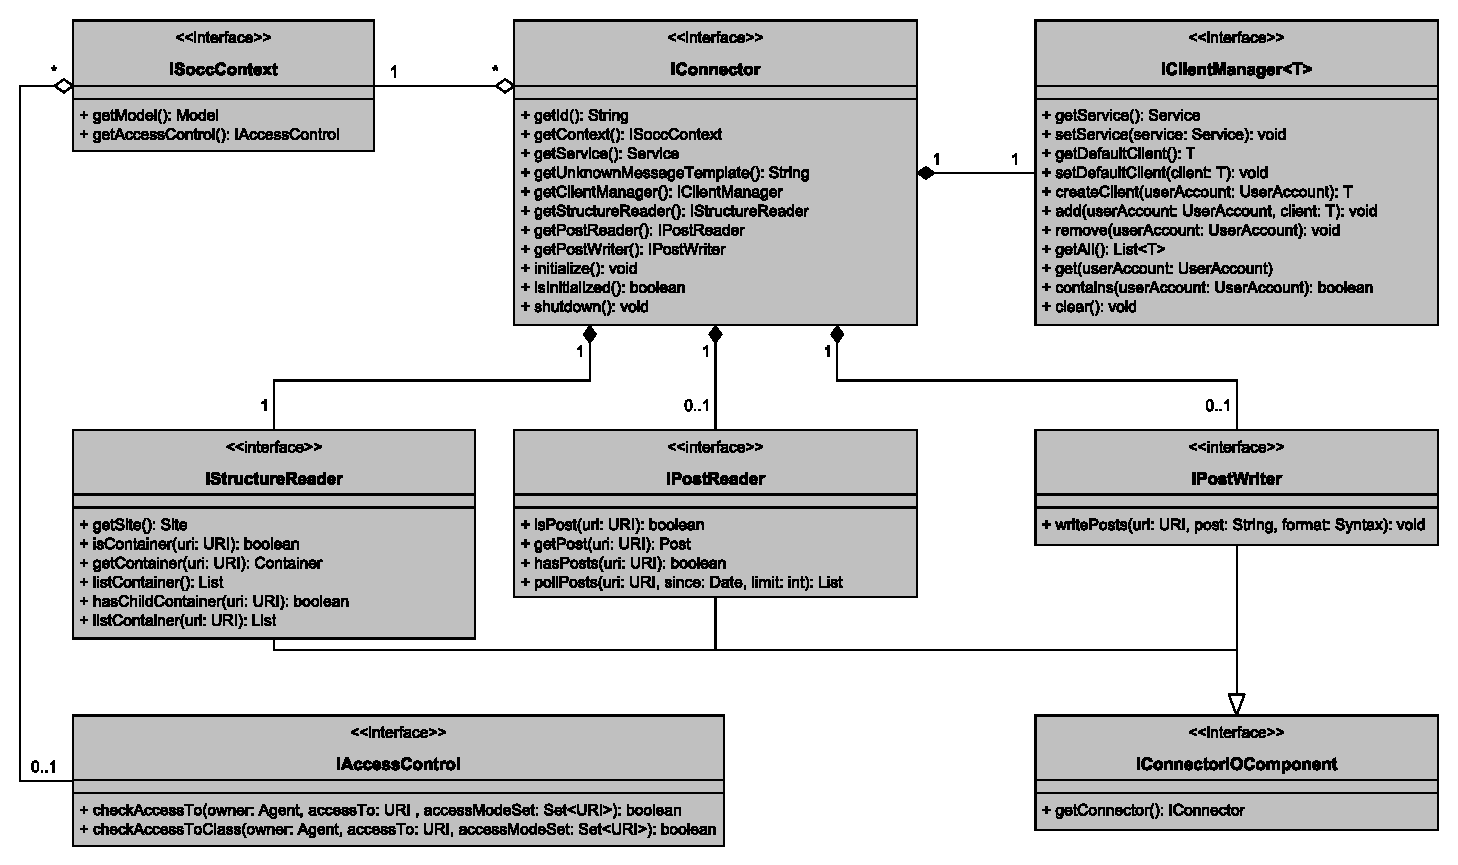
\includegraphics[
        width=9cm,
        keepaspectratio=true,
        clip=true,
        trim= 243 129 255 206]
    {assets/images/socc_uml_classdiagram}
    \caption{PostReader}
    \label{fig:uml_post_reader}
\end{wrapfigure}

Der \texttt{PostReader} dient als Schnittstelle für das Lesen geschriebener Beiträge innerhalb eines Containers oder der Kommentare auf einen anderen Beitrag. Er stellt nach außen hin Funktionen bereit mit denen entweder ein einzelner Beitrag oder alle Beiträge, die bestimmte Kriterien erfüllen, gelesen werden können. Bevor ein Beitrag zurück gegeben wird, müssen die Methoden prüfen, ob der Autor eines Beitrag das Lesen für diesen erlaubt hat. Falls nicht, wird der Beitrag aus der Ergebnisliste gestrichen und nicht zurückgegeben. Die Funktionsweise der einzelnen Methoden ist wie folgt:

\begin{description}
    \item[\texttt{isPost(uri: URI)}] kann zur Überprüfung eingesetzt werden, ob sich hinter einer URI ein Beitrag befindet.

    \item[\texttt{getPost(uri: URI)}] ist dazu gedacht einen einzelnen Beitrag anhand seiner URI zu lesen. Sie liefert dann den Beitrag als Objekt der SIOC-Klasse Post zurück.

    \item[\texttt{hasPost(uri: URI)}] funktioniert ähnlich wie isPost, überprüft aber ob sich hinter der angegeben URI noch weitere Beiträge befinden können. 

    \item[\texttt{pollPosts(uri: URI, since: Date, limit: int)}] ist eine Methode die alle Beiträge hinter eine URI liest welche die gegeben Kriterien erfüllen. Insgesamt erhält diese Methode drei Parameter. Der Erste ist eine URI die den Ort angibt von der die Beiträge gelesen werden sollen. Mit dem zweiten Parameter kann ein Zeitpunkt angegeben werden, ab dem ein zu lesender Beitrag geschrieben sein muss. Zum Beispiel der Zeitpunkt als diese Methode das letzte mal aufgerufen wurde, um alle Beiträge die danach geschrieben wurden zu lesen. Der letzte Parameter gibt eine obere Schranke an, wie viele Beiträge maximal pro Aufruf dieser Methode gelesen werden dürfen. Ist dieses Limit erreicht, werden keine weiteren Beiträge in die Ergebnisliste aufgenommen.
\end{description}

% subsubsection postreader (end)

\subsection{PostWriter} % (fold)
\label{sub:postwriter}
%% korrigiert am 2013-09-26 21:35

In Abbildung \ref{fig:postwriter_sequenzdiagramm} ist ein Sequenzdiagramm der PostWriter Komponente zu sehen. Dort ist visualisiert, welche Schritte für das stellvertretende Schreiben von Beiträgen eines Benutzers unternommen werden müssen. Soll nun ein Beitrag in Plattform des Connectors geschrieben werden, wird die Methode \texttt{writePost(URI, String, Syntax)} mit dem Zielort als URI, dem Beitrag als serialisiertes RDF Objekt und dem verwendeten Serialisierungsformat aufgerufen. Es beginnt damit, dass zuerst nach einem Benutzerkonto des Beitragautors für die Plattform des aktuellen Connectors gesucht wird. Dieser sollte im Idealfall im Triplestore des Connectors nach dem im Abschnitt \ref{sub:benutzerdaten} Schema vorliegen. Mit diesem Benutzerkonto, in Form der Klasse UserAccount von SIOC, kann dann vom ClientManager ein Client für die verwendete API geholt werden. Sollte die Suche negativ verlaufen, steht noch der Defaultclient zur Verfügung. 
Bevor der Beitrag aber geschrieben werden kann, muss nachgeschaut werden, ob eine Erlaubnis für das Schreiben mit dem Client vorliegt. Ist dies der Fall kann der Beitrag in das von der API verwendete Format konvertiert und an die richtige Stellen der Plattform geschrieben werden.

\begin{minipage}{\textwidth}
    \centering
    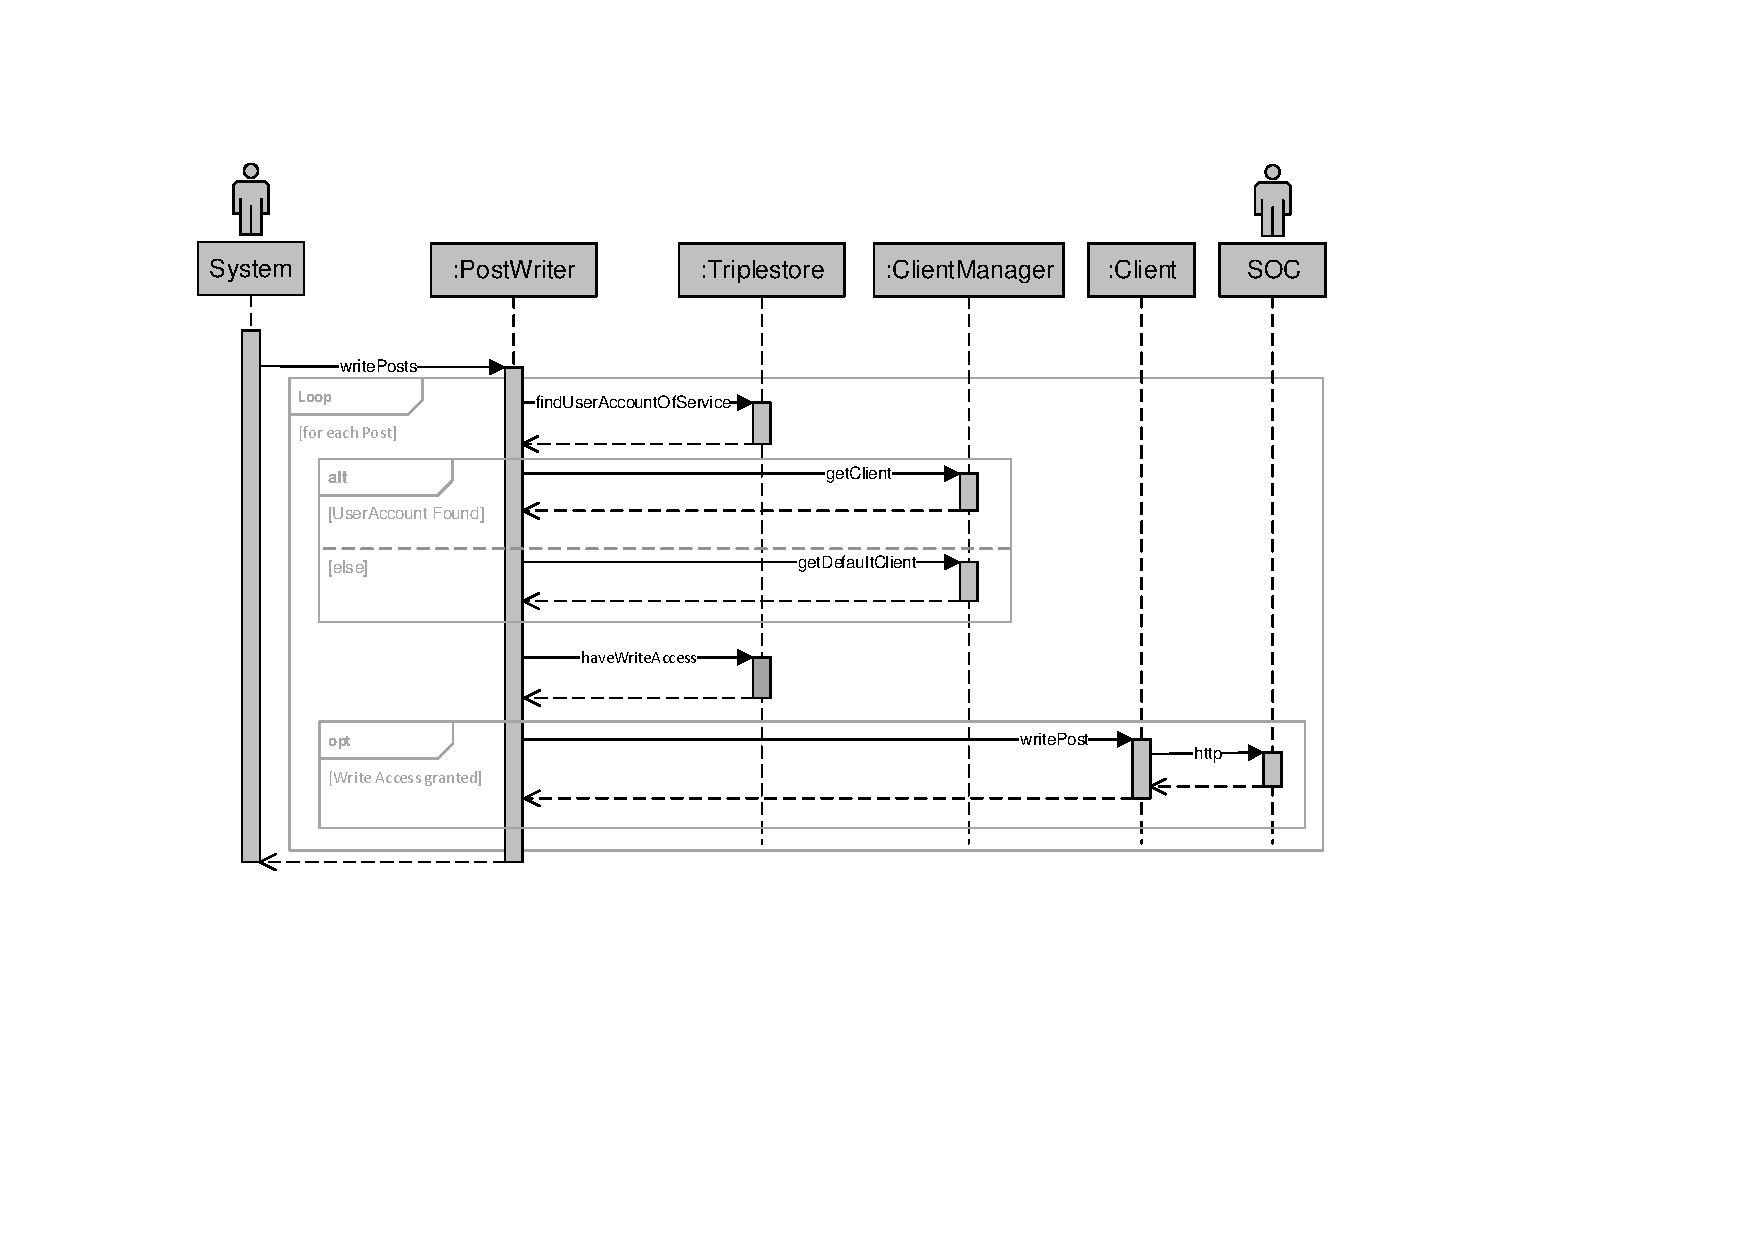
\includegraphics[
        width=\textwidth,
        keepaspectratio=true,
        clip=true,
        trim= 90 180 220 75]
    {assets/images/postwriter_sequencediagram}
    \captionof{figure}{UML Sequenzdiagramm eines PostWriters}
    \label{fig:postwriter_sequenzdiagramm}
\end{minipage}

% subsubsection postwriter (end)

% subsection connector_aufbau (end)

% section social_online_community_connectors (end)

\section{SOCC-Camel} % (fold)
\label{sec:socc_camel}
%% korrigiert am 2013-09-26 22:04

\emph{SOCC-Camel} ist eine Modul der SOCC für die Integration von Connectoren in Camel. Durch dieses ist auf flexible Weise möglich die gelesenen Beiträge von einer Plattform über die Connectoren in eine andere zu schreiben. Abbildung \ref{fig:uebersicht_socc_camel} zeigt SOCC-Camel als EIP-Diagramm. 

\begin{minipage}{\textwidth}
    \centering
     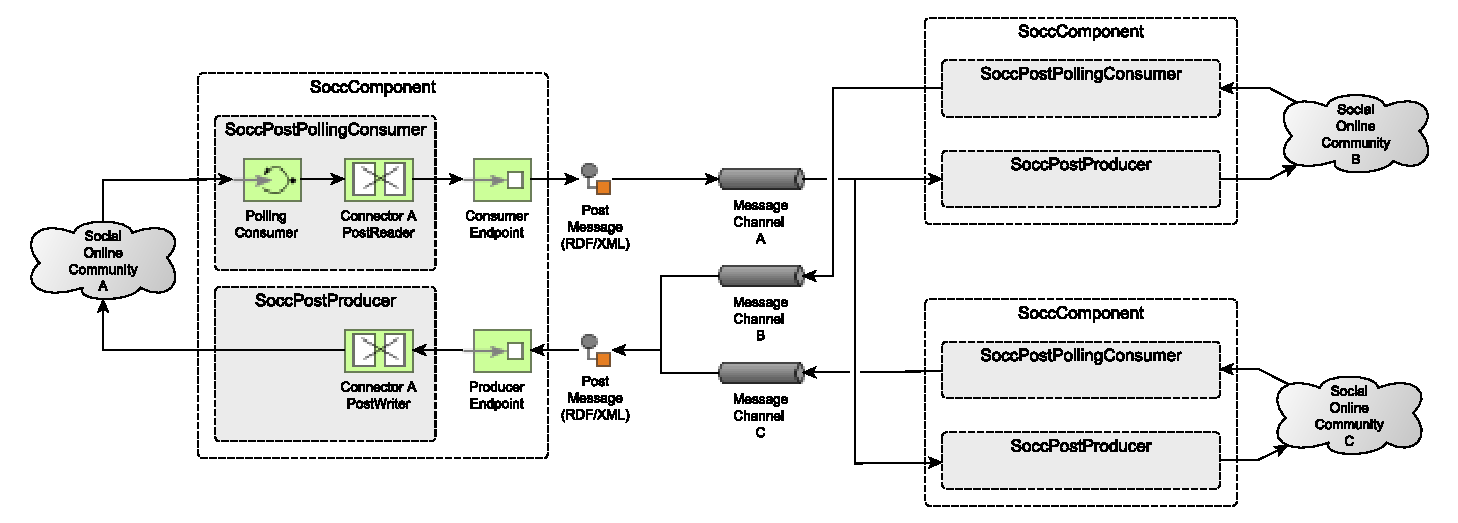
\includegraphics[
        width=\textwidth,
        keepaspectratio=true]
        {assets/images/socc_camel_overview}
    \captionof{figure}{Übersicht des Socc-Camel Moduls in EIP-Notation}
    \label{fig:uebersicht_socc_camel}
\end{minipage}

Hauptklasse dieses Moduls ist \texttt{SoccComponent}. Sie ist für die Verwaltung von Connectoren und Erstellen der Endpunkte für Camel zuständig. Von dieser Klasse muss zuerst ein Objekt erzeugt und ein SoccContext mit dem Tripelstore und alle Informationen für die Connectoren wie ConnectorConfigs Benutzerkonten und Services übergeben werden. Also alle Daten die in Anschnitt \ref{sec:konfiguration} beschrieben wurden. Das SoccComponent Objekt wird dann unter einen frei wählbaren Namen in Camel registriert. Als Namen ist \enquote(socc) aber vorzuziehen.  Nun kann wie in Abschnitt \ref{ssub:apache_camel} mit dieser Komponente Routen erstellt werden. Die URIs für die Konfiguration der Endpunkte mit SOCC-Camel habe dazu den folgenden Aufbau:

\begin{lstlisting}[
    caption={SOCC-Camel Konfigurations URI}\label{lst:socc_camel_uri},
    captionpos=t]
socc://{connectorId}?uri={targetUri}[&{parameter}...]
\end{lstlisting}

Der Anfang der URI mit \enquote{socc://} sagt Camel, dass es für diesen Endpunkt die Komponente benutzten soll, die vorher unter dem Namen \enquote{socc} registriert wurde - also die SoccComponent. Für den Platzhalter \enquote{\{connectorId\}} muss eine gültige ID eines Connectors sein, dessen Konfigurationsdaten im TripleStore hinterlegt wurden. Über den Parameter \enquote{uri} wird dann die Quell- beziehungsweise Ziel-URI für den Connector angegeben, von der er Beiträge lesen soll. Je nach Endpunkt können dann noch weitere Parameter angegeben werden. So ein Endpunkt wird in SOCC-Camel durch die Klasse \texttt{SoccEndpoint} modelliert (nicht explizit in der Abbildung angegeben) und leitet sich von der Klasse \texttt{ScheduledPollEndpoint}, die das Verwenden der folgenden \texttt{SoccPostPollConsumer} Klasse vereinfacht.

\subsection{SoccPostPollConsumer} % (fold)
\label{sub:soccpostpollingconsumer}

Wird ein Endpunk mit der Absicht zum Lesen von Beiträgen erstellt, erzeugt die Klasse SoccComponent ein Objekt der Klasse SoccPostPollConsumer und übergibt im die Parameter aus der Konfigurations-URI. Da SoccPostPollingConsumer sich von der Klasse ScheduledPollConsumer ableitet, ist es über dem Parameter \texttt{delay} möglich in periodischen Abständen das Lesen von Beiträgen auszuführen. Die Angabe erfolgt dabei in Millisekunden. Der Parameter \texttt{limit} entspricht dabei den gleichnamigen Argument der Methode \texttt{pollPosts(\dots)} des PostReaders aus Abschnitt \ref{sub:postreader}. Das dort noch fehlende Argument \texttt{since}, für das Datum, ab wann ein Beitrag als neu gilt, holt sich der SoccPostPollConsumer aus den im TripleStore gespeicherten Daten. Da dort in den Strukturdaten gespeichert wird, wann der letzte Beitrag eines Threads oder der letzte Kommentar auf einen Beitrag gespeichert wird. Alle neuen, gelesenen Beiträge werden am Ende in das RDF/XML-Format serialisiert und als Nachricht an Camel übergeben, welches es dann anhand der festgelegten Routen weiterleitet. Damit andere Komponenten diese Nachricht wieder korrekt de-serialisieren können, muss der Nachricht noch ein Header mit dem Schlüssel \enquote{Content-Type} und dem MIME-Type\footnote{ Multipurpose Internet Mail Extension - Types: \url{http://tools.ietf.org/html/rfc2046}} vom RDF/XML \enquote{application/rdf+xml} mitgegeben werden.

% subsection soccpostpollconsumer (end)

\subsection{SoccPostProducer} % (fold)
\label{sub:soccpostproducer}

Der SoccPostProducer ist das Gegenstück zum SoccPostPollConsumer. Er ist der Endpunkt der zum Schreiben von Beiträgen in die Plattform des Connectors von der Klasse SoccComponent erzeugt wird. Intern verwendet er den PostWriter des betreffenden Connetors und leitet den Inhalt der Nachricht an diese weiter. Außer der Angabe über die Ziel-URI erhält der SoccPostProducer keine weiteren Parameter über die Konfigurations-URI. Der SoccPostProducer überprüft auch ob ein gültiger MIME-Type angeben wurde. Akzeptiert wird auf jeden Fall \enquote{application/rdf+xml} für RDF/XML. Je nach verwendeten Adapter für RDF2Go können auch \enquote{"application/x-turtle"} für Turtle oder \enquote{application/rdf+json} für RDFJson\footnote{\url{https://dvcs.w3.org/hg/rdf/raw-file/default/rdf-json/index.html}} verwendet werden.

% subsection soccpostproducer (end)

% section socc_camel (end)

% chapter eigener_ansatz_social_online_community_connectors_socc_ (end)
